\section{Motivation}
We may classify filters as linear or non-linear. A filter is said to be \textit{linear} if the filtered, smoothed, or predicted quantity at the output of the filter is a \textit{linear function of the observations applied to the filter input}. Otherwise, the filter is nonlinear.
\subsection{Linear Filter}
$C_2$ in graphic \ref{linearfilter} can be tuned $\rightarrow$ programmable filter (due to changeable parameters). Note that this is not an Adaptive Filter yet, just a programmable one.\\
E.g. Bandpass with changeable frequency but same bandwidth (you have to change all: C, R and L!).
\begin{figure}[H]
	\centering
	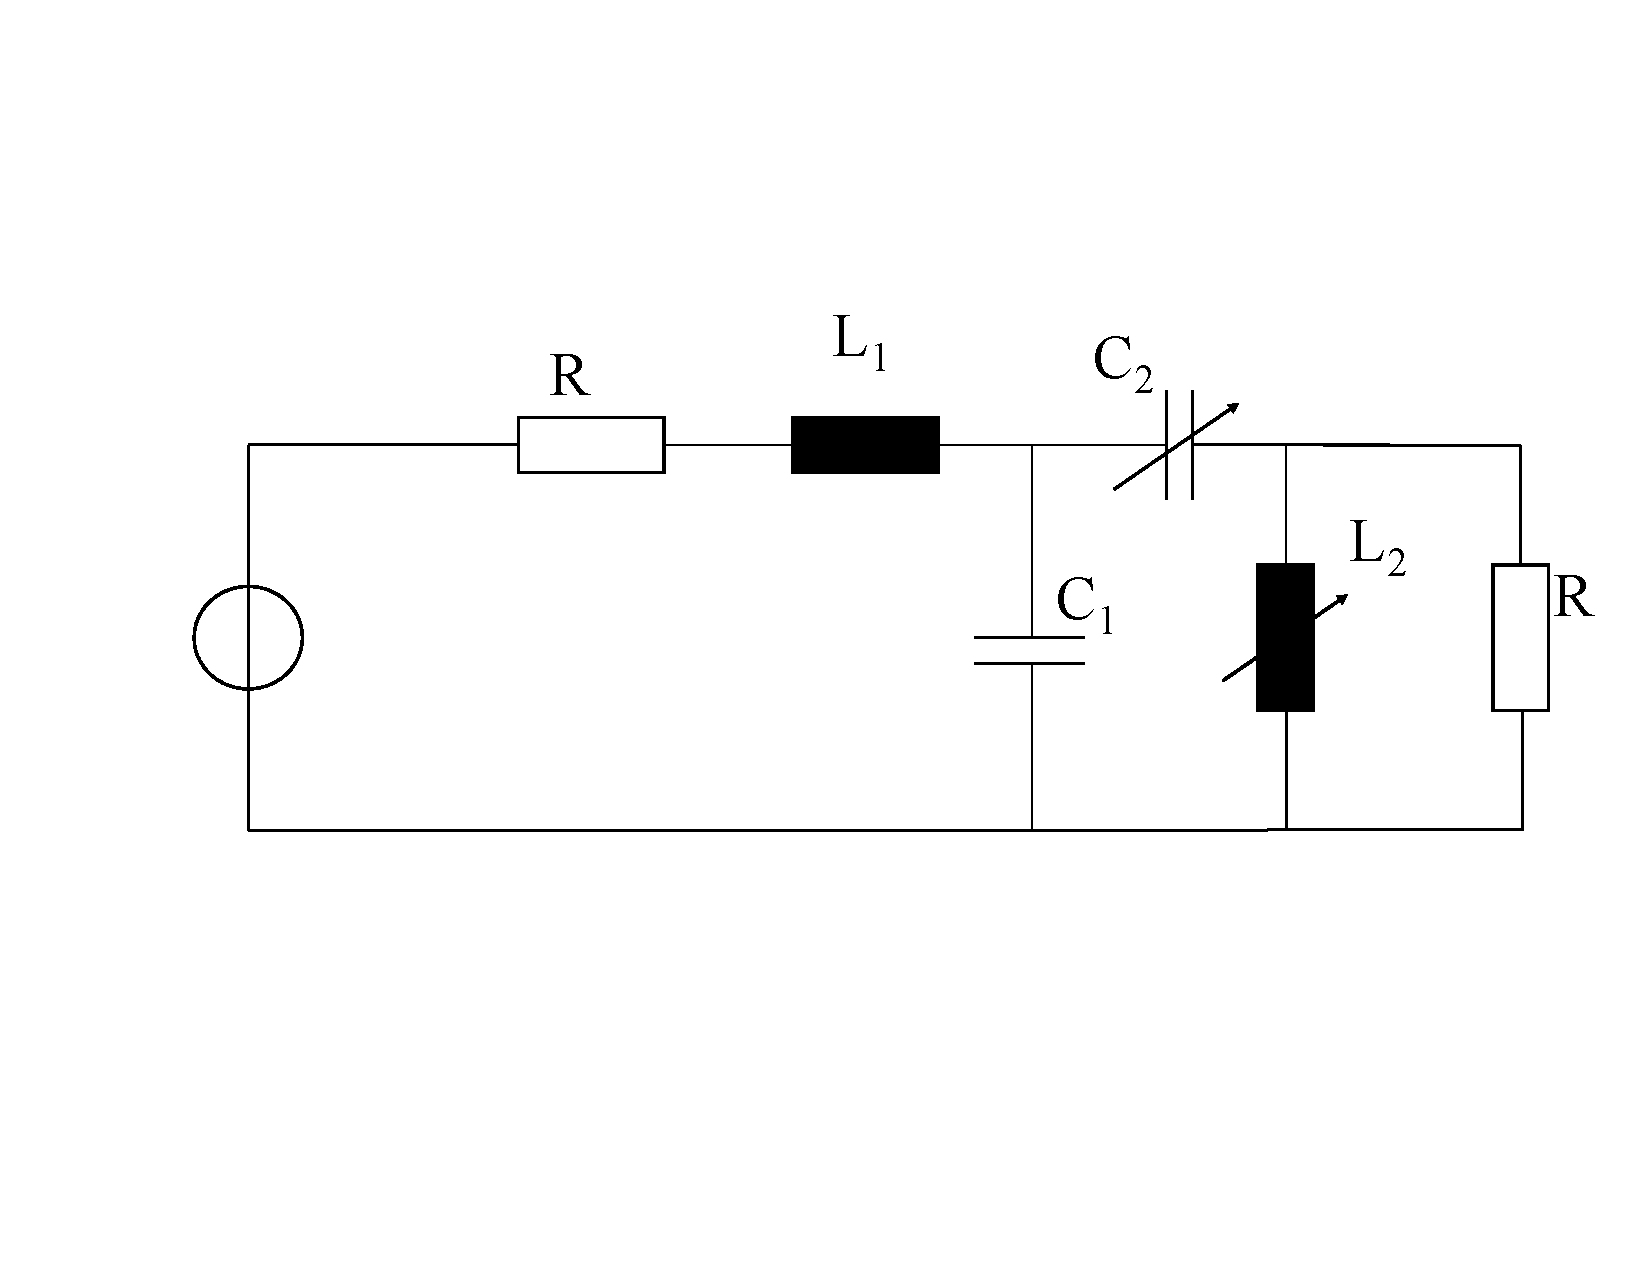
\includegraphics[scale=0.5, trim =1cm 7cm 1cm 5cm,clip ]{linear_filter.pdf}
	\caption{Linear Filter, fixed parameters}
	\label{linearfilter} 
\end{figure}
\subsection{Discrete Filter}
\begin{figure}[H]
	\centering
	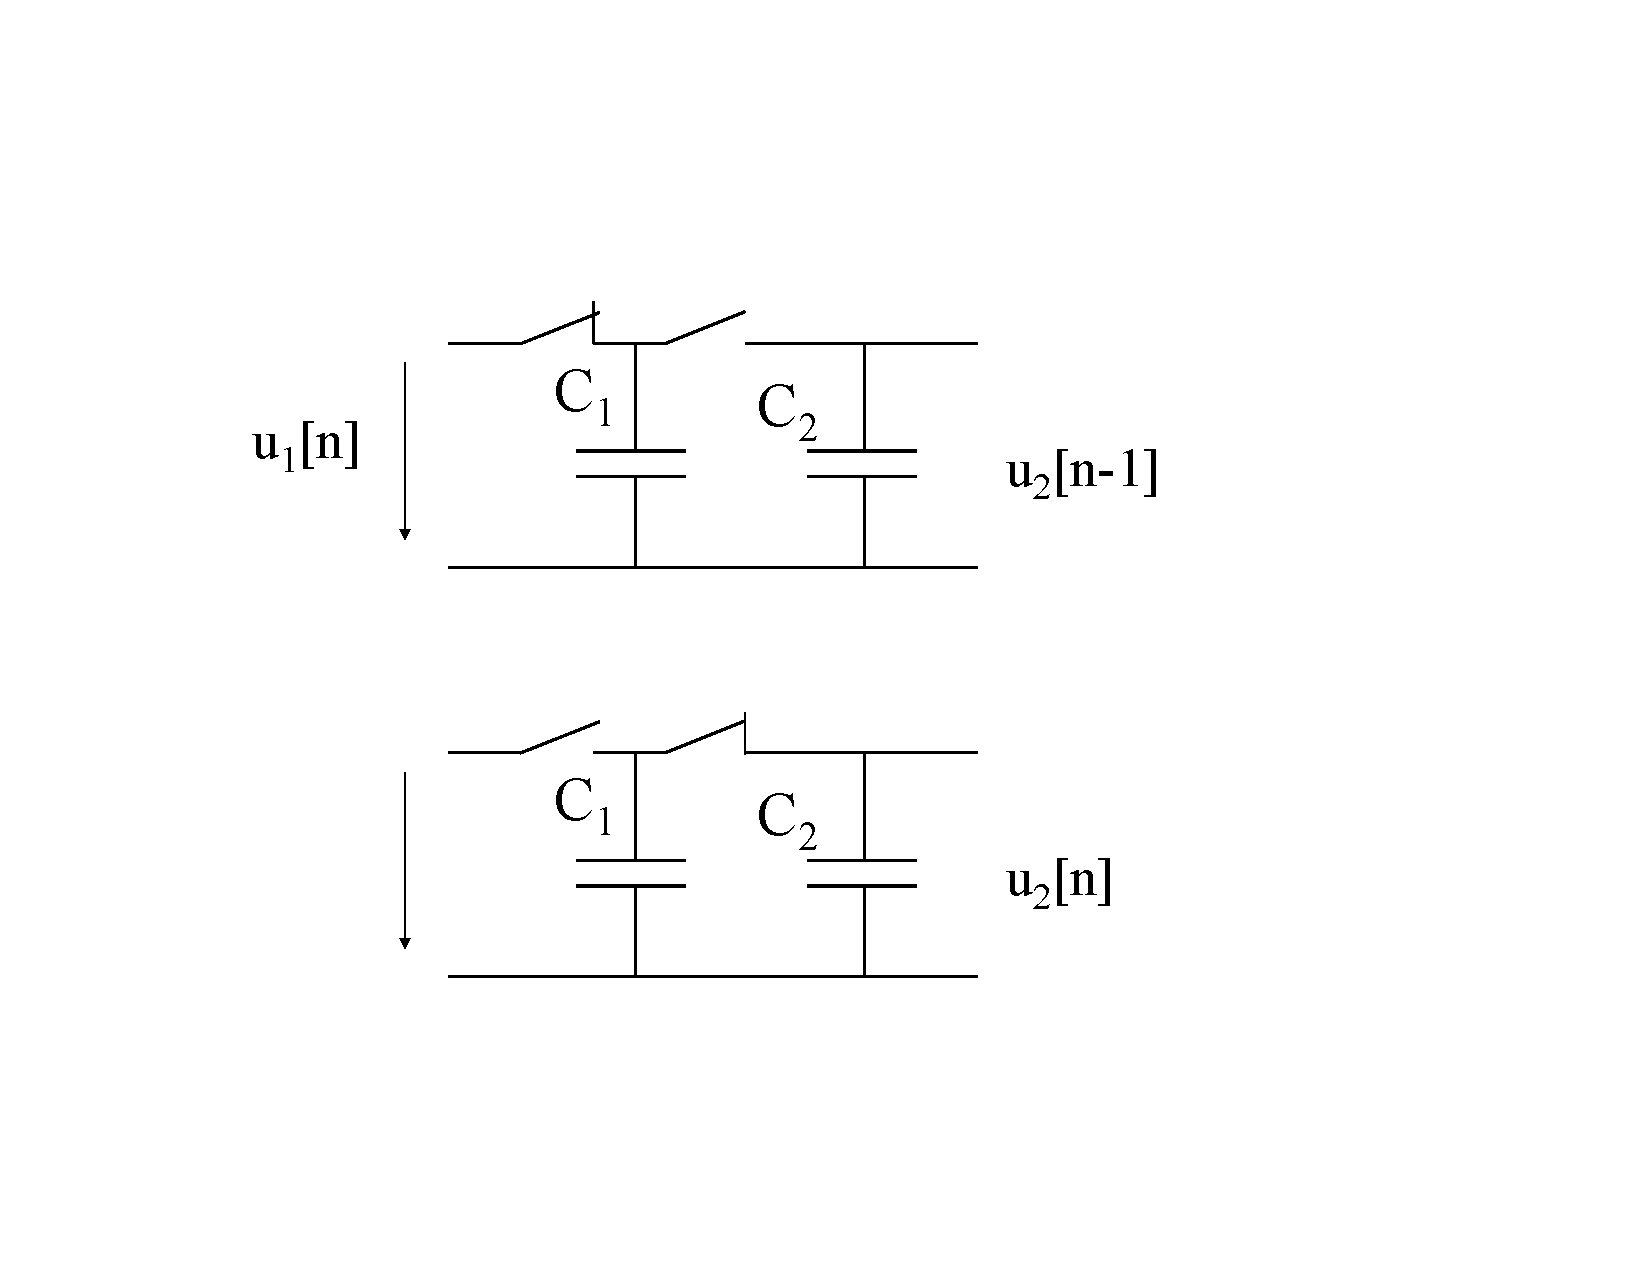
\includegraphics[scale=0.5, trim =3cm 5cm 6cm 5cm,clip ]{discrete_filter.pdf}
	\caption{One open, one closed, discrete time filter}
	\label{discretefilter} 
\end{figure}
\subsubsection{IIR-Filter}
Infinite impulse response (IIR) is a property applying to many linear time-invariant systems. Common examples of linear time-invariant systems are most electronic and digital filters. Systems with this property are known as IIR systems or IIR filters, and are distinguished by having an impulse response which does not become exactly zero past a certain point, but continues indefinitely. This is in contrast to a finite impulse response (FIR) in which the impulse response h(t) does become exactly zero at times $t > T$ for some finite T, thus being of finite duration.
The discrete filter in picture \ref{discretefilter} is defined by:\\ 
$C_1\cdot u_1[n] + C_2\cdot u_2[n-1] = (C_1+C_2 )u_2[n]$\\ 
$u_2[n]= \underbrace{\frac{C_2}{C_1+C_2}}_{a}\cdot u_2[n-1] + \underbrace{\frac{C_1}{C_1+C_2}}_{1-a}\cdot u_1[n]$\\
It's impulse response is given by table \ref{tab:prog_filter_Impulse_Resp}. As can be seen coefficient $a$ allows us to change the filter's impulse response and therefore to program the filter. Figure \ref{discreteeasy} shows a block diagram for such an easy, programmable discrete filter. From this block diagram it can be seen immediately that this filter is an IIR-Filter and can therefor be unstable.
\begin{figure}[H]
	\centering
	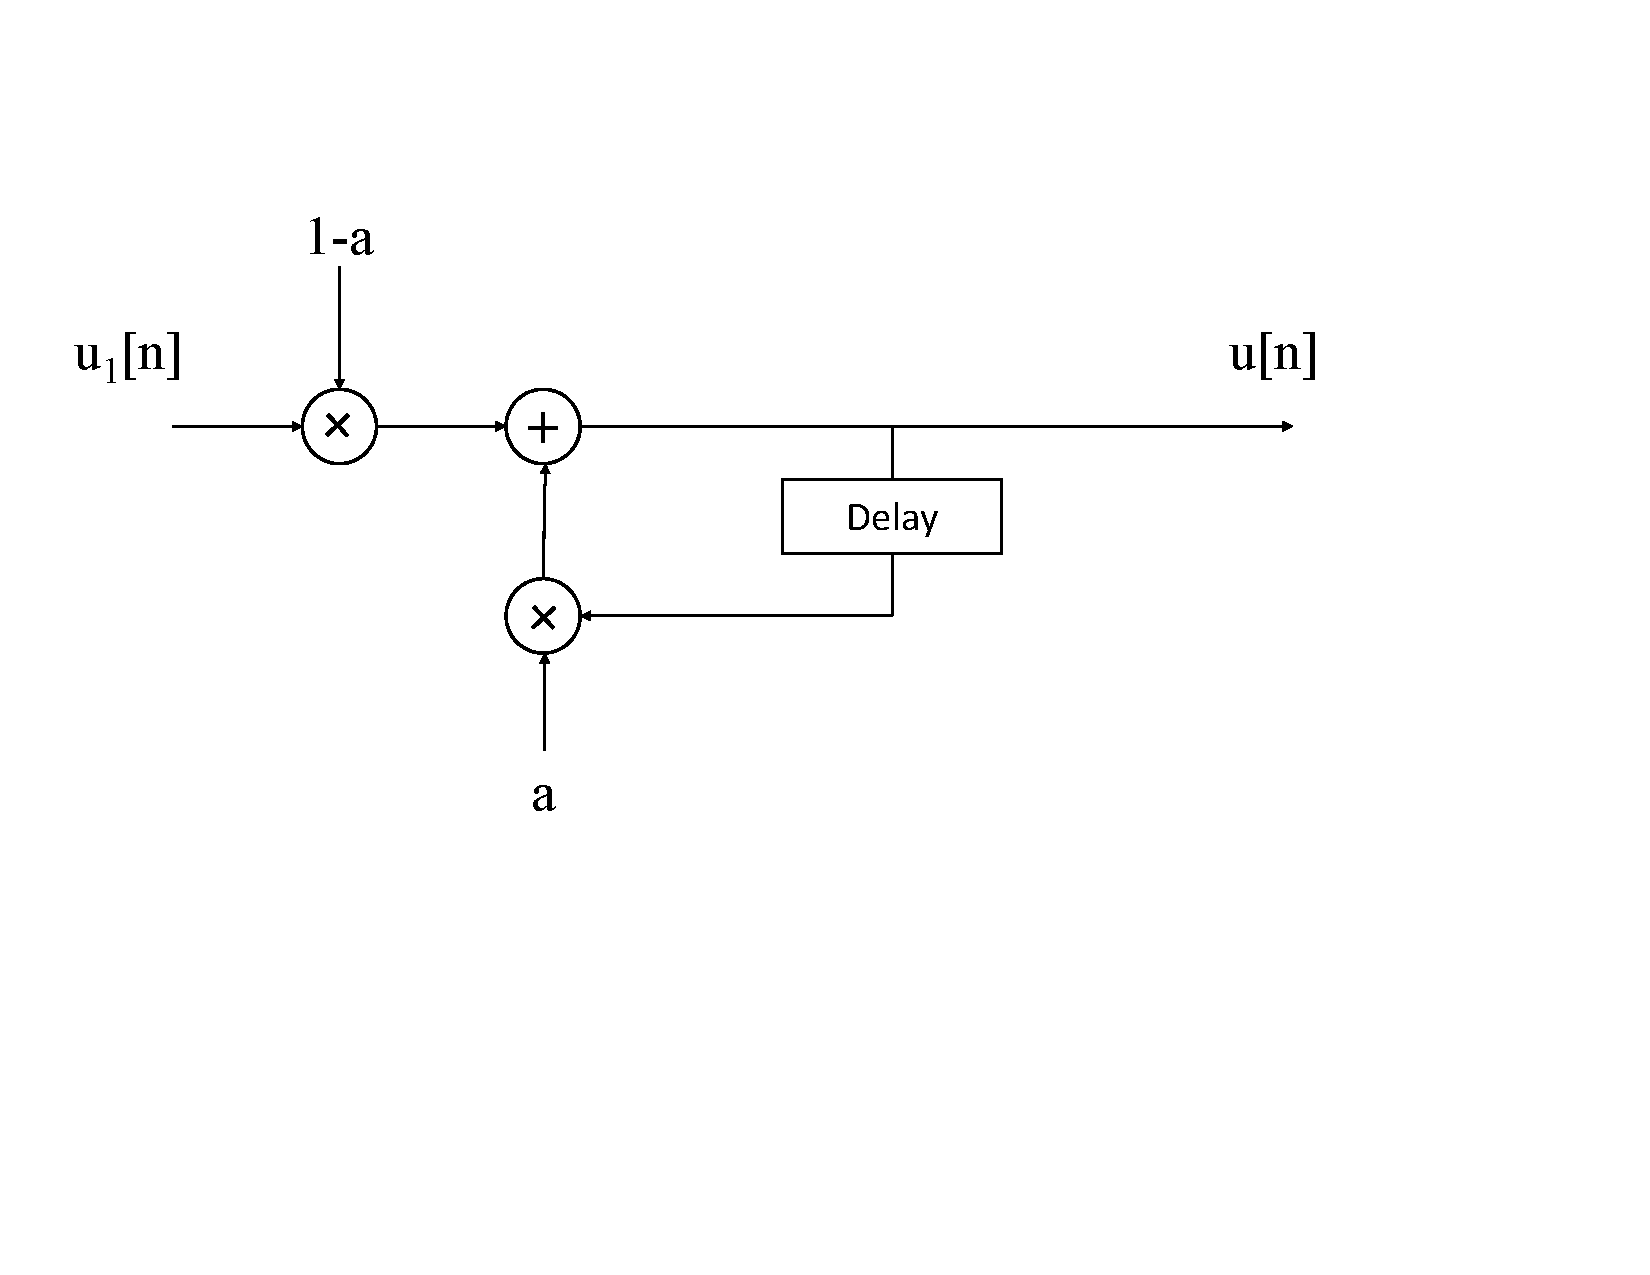
\includegraphics[scale=0.5, trim=1cm 7cm 3cm 2cm,clip]{discrete_easy.pdf}
	\caption{Discrete, easy to program filter}
	\label{discreteeasy} 
\end{figure}

\begin{table}
	\caption{discrete filter - Impulse Response }	
	\label{tab:prog_filter_Impulse_Resp}
	\centering
\begin{tabular}[H]{|c|cccccc|}
\hline
	n & $\leq$ 0 & 0 &1 &2 & ... &k\\
	\hline
	$u_1[n]$& 0 & 1 & 0 & 0 & ... &0\\
	$u_2[n]$& 0 & $1-a$ & $a(1-a)$&$ a^2(1a) $& ... & $a^k (1-a)$\\
	\hline
\end{tabular}
\end{table}

\textbf{Caution!} Proof of stability required! \\ $|a| \geq 1 \rightarrow $ instable \pfeil $|a| \leq 1 \rightarrow$ stable.
\begin{figure}[H]
	\centering
	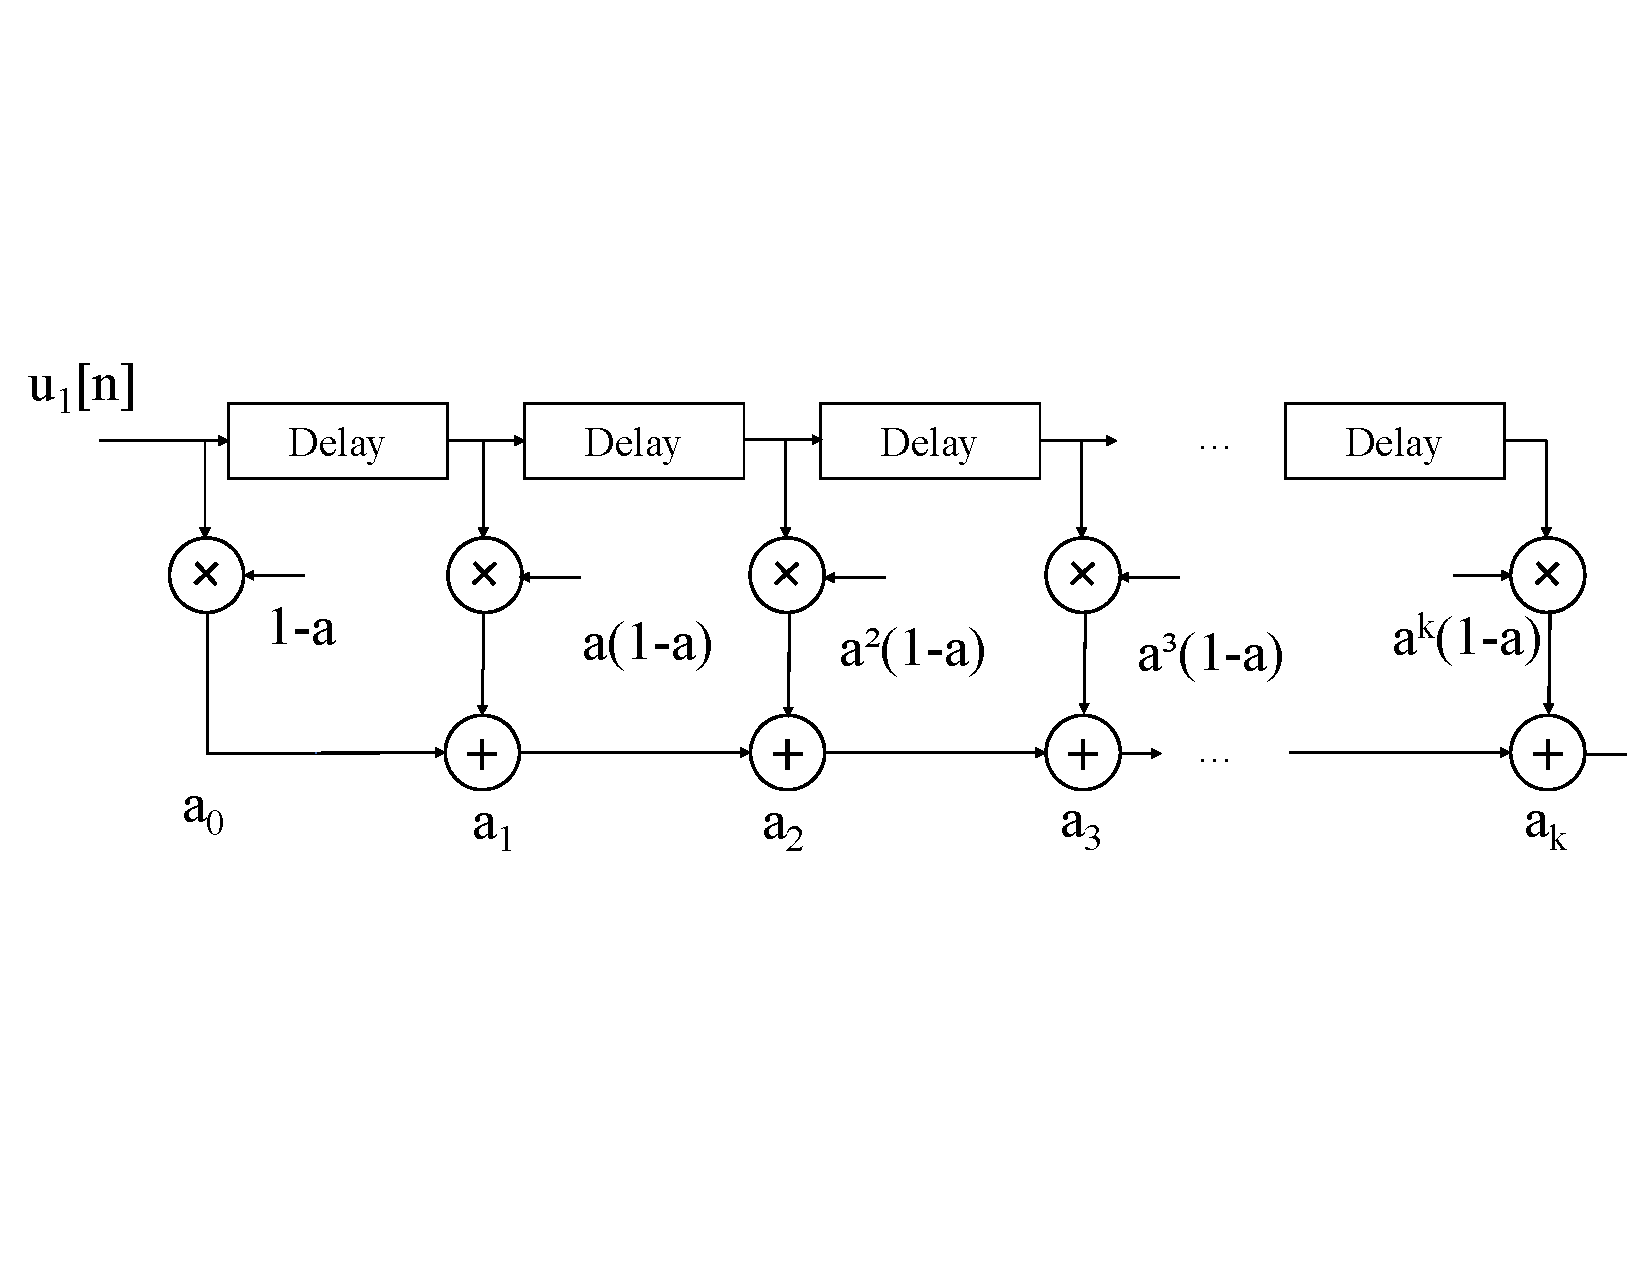
\includegraphics[scale=0.5, trim=0cm 5cm 0cm 5cm,clip]{delay_filter.pdf}
	\caption{Linear adaptive filter (tapped delay line)}
	\label{delayfilter} 
\end{figure}

\subsubsection{FIR-Filter}
To overcome the stability problems an FIR-filter can be used instead. FIR-Filters are always stable.
Suitable for adaptive filters but it's an approximation \pfeil finite \\
Structure: tapped delay line \\
linear: neither delay only coefficient are dependent in input signal. $\rightarrow$ linear adaptive filter, see picture \ref{delayfilter}.\\ \\

\textbf{Delays of 1 clock cycle:}\\
$D\cdot x[n] = x[n-1]$\\ \\
\textbf{Delay of 2 clock cycles:}\\
$\underbrace{DD}_{D^2}\cdot x[n] = D \cdot x[n-1] = x[n-2]= D^2\cdot x[n] $\\ \\

\textbf{Fractional delay:}\\
$F \cdot x(n) = x(n-\frac{1}{2})$\\
$FF \cdot x(n) = F \cdot x(n-\frac{1}{2}) = x[n-1] = D \cdot x[n]$\\
$F^2 = FF  	\equiv D ; F= \sqrt{D} = D^{\frac{1}{2}}$\\
$D^{\frac{1}{2}} \cdot D^{\frac{1}{2}} = D^{\frac{1}{2}+\frac{1}{2}} = D' =D$ \\
Developed using a Taylor series: $D^{\frac{1}{2}} \approx  1+\frac{1}{2}(D-1)+ \frac{1}{8}(D-1)^2 = \frac{3}{8}+\frac{3}{4}\cdot D + \frac{1}{8} D^2$\\
The filter in graphic \ref{delayfilter1_2} shows the shifting of the signal by $\frac{1}{2}$.
\begin{figure}[H]
	\centering
	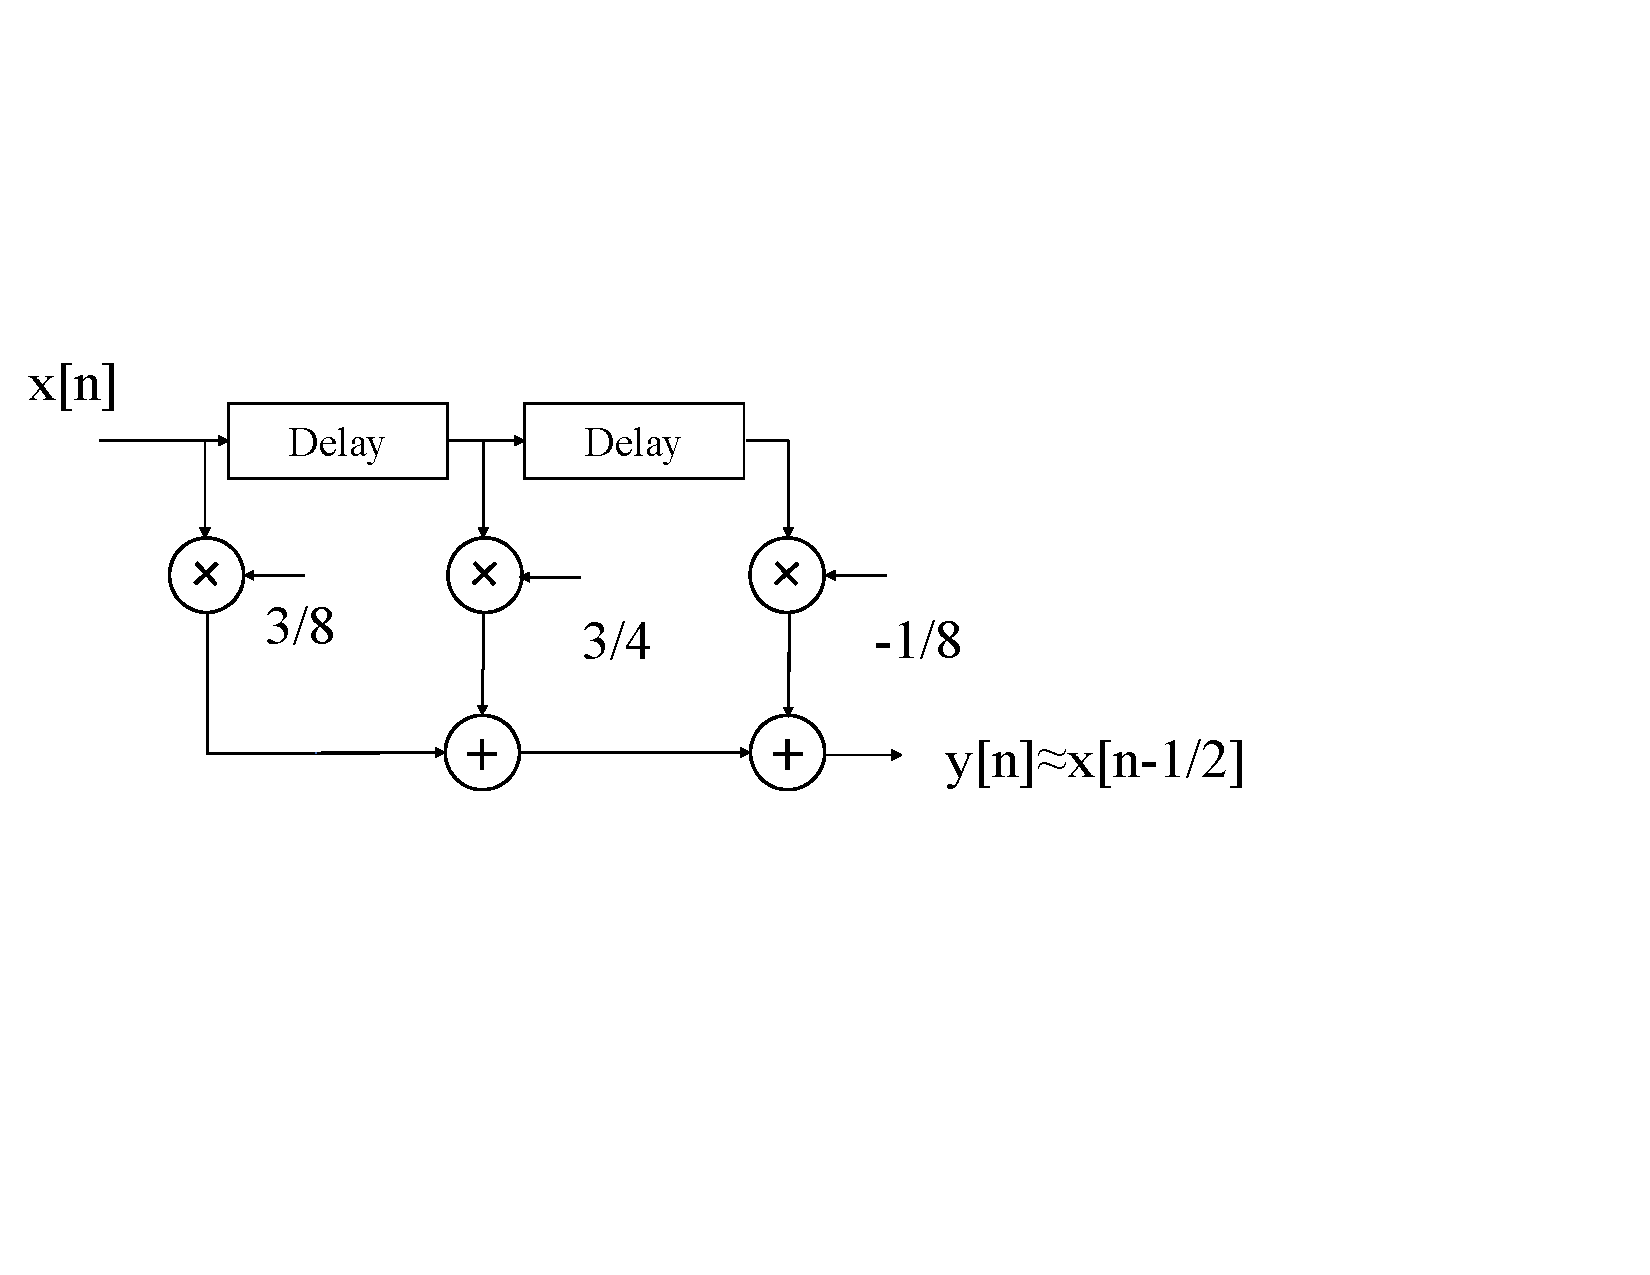
\includegraphics[scale=0.5, trim=0cm 8cm 0cm 6cm, clip]{delay_1_2.pdf}
	\caption{Used for synchronization of receiver and transmitter}
	\label{delayfilter1_2} 
\end{figure}

A fractional delay $y[n] \approx u[n-a] $ for $0 \leq a \leq 1$ \\
$y[n] = a_0 \cdot u[n] + a_1 \cdot u[n-1] + a_2 \cdot u[n-2] $ with $ a_0 = \frac{1}{2} (a^2 + 3a + 2)$ and $a_1 = (2-a)a$ and $a_2= \frac{1}{2} (a-1) a $\\

\begin{figure}[H]
	\centering
	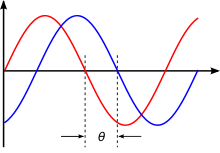
\includegraphics{phaseshift.png}
	\caption{Phase-shift for $\theta$}
	\label{phaseshift} 
\end{figure}

\textbf{Example:} $a=\frac{1}{2} \quad u[n]=sin(\frac{n}{2})$\\
A node is passing \[ S= \sum_{i=1}^2 |a_i|^2 = \frac{1}{2}a^4 - 6a^3 +\frac{5}{2} a^2 - 3a+1\] remains $\leqq 1$ only for $0\leq a\leq 2$. For $a < 0  $ or $a > 2$ it grows unboundenly.\\ This is relevant, since uncorrelated noise at the input leads to an output which mean square is proportional to S. Thus, $a < 2$ or $a < 0$ are possible, but with a (huge) noise penalty. The mean squared output noise is minimum for $a = 1-\frac{1}{\sqrt{2}} \approx 0,3$
\begin{figure}[H]
	\centering
	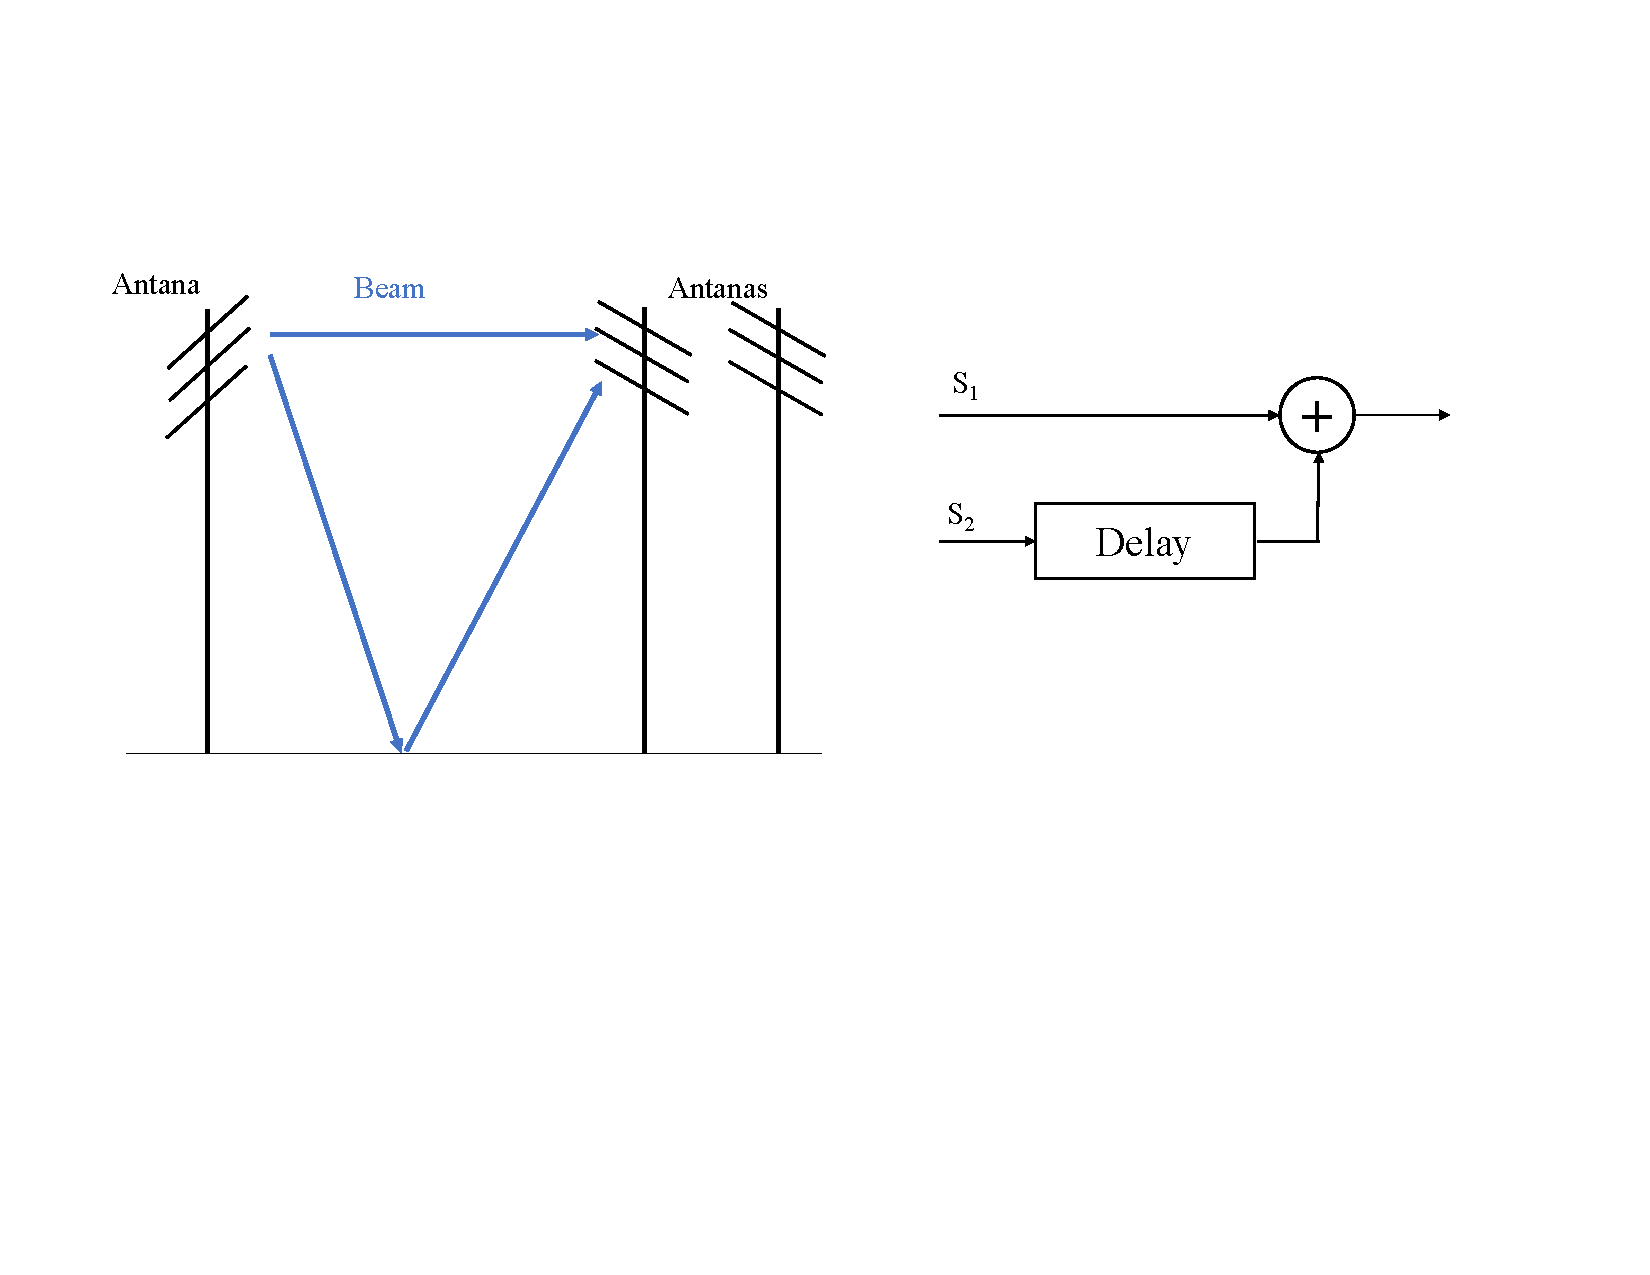
\includegraphics[scale=0.5, trim=1cm 8cm 1cm 4cm, clip]{antenna.pdf}
	\caption{2 signals, but delayed.}
	\label{delayedsignal} 
\end{figure}
The sketch in figure \ref{delayedsignal} shows a signal which travels trough two paths from the transmitter to the receiver. One signal is faster (has a shorter way) than the other. To be able to add the two signals the faster one has to be delayed and since the delay between the two signals is (usually) not an integer the fractional delay is needed here.\\
 \pfeil After delaying the faster one, they're only different in their amplitude and can be added. (Otherwise we get fading effects.)

\subsection{Principle Structure of an Adaptive Filter}


\begin{figure}[H]
	\centering
	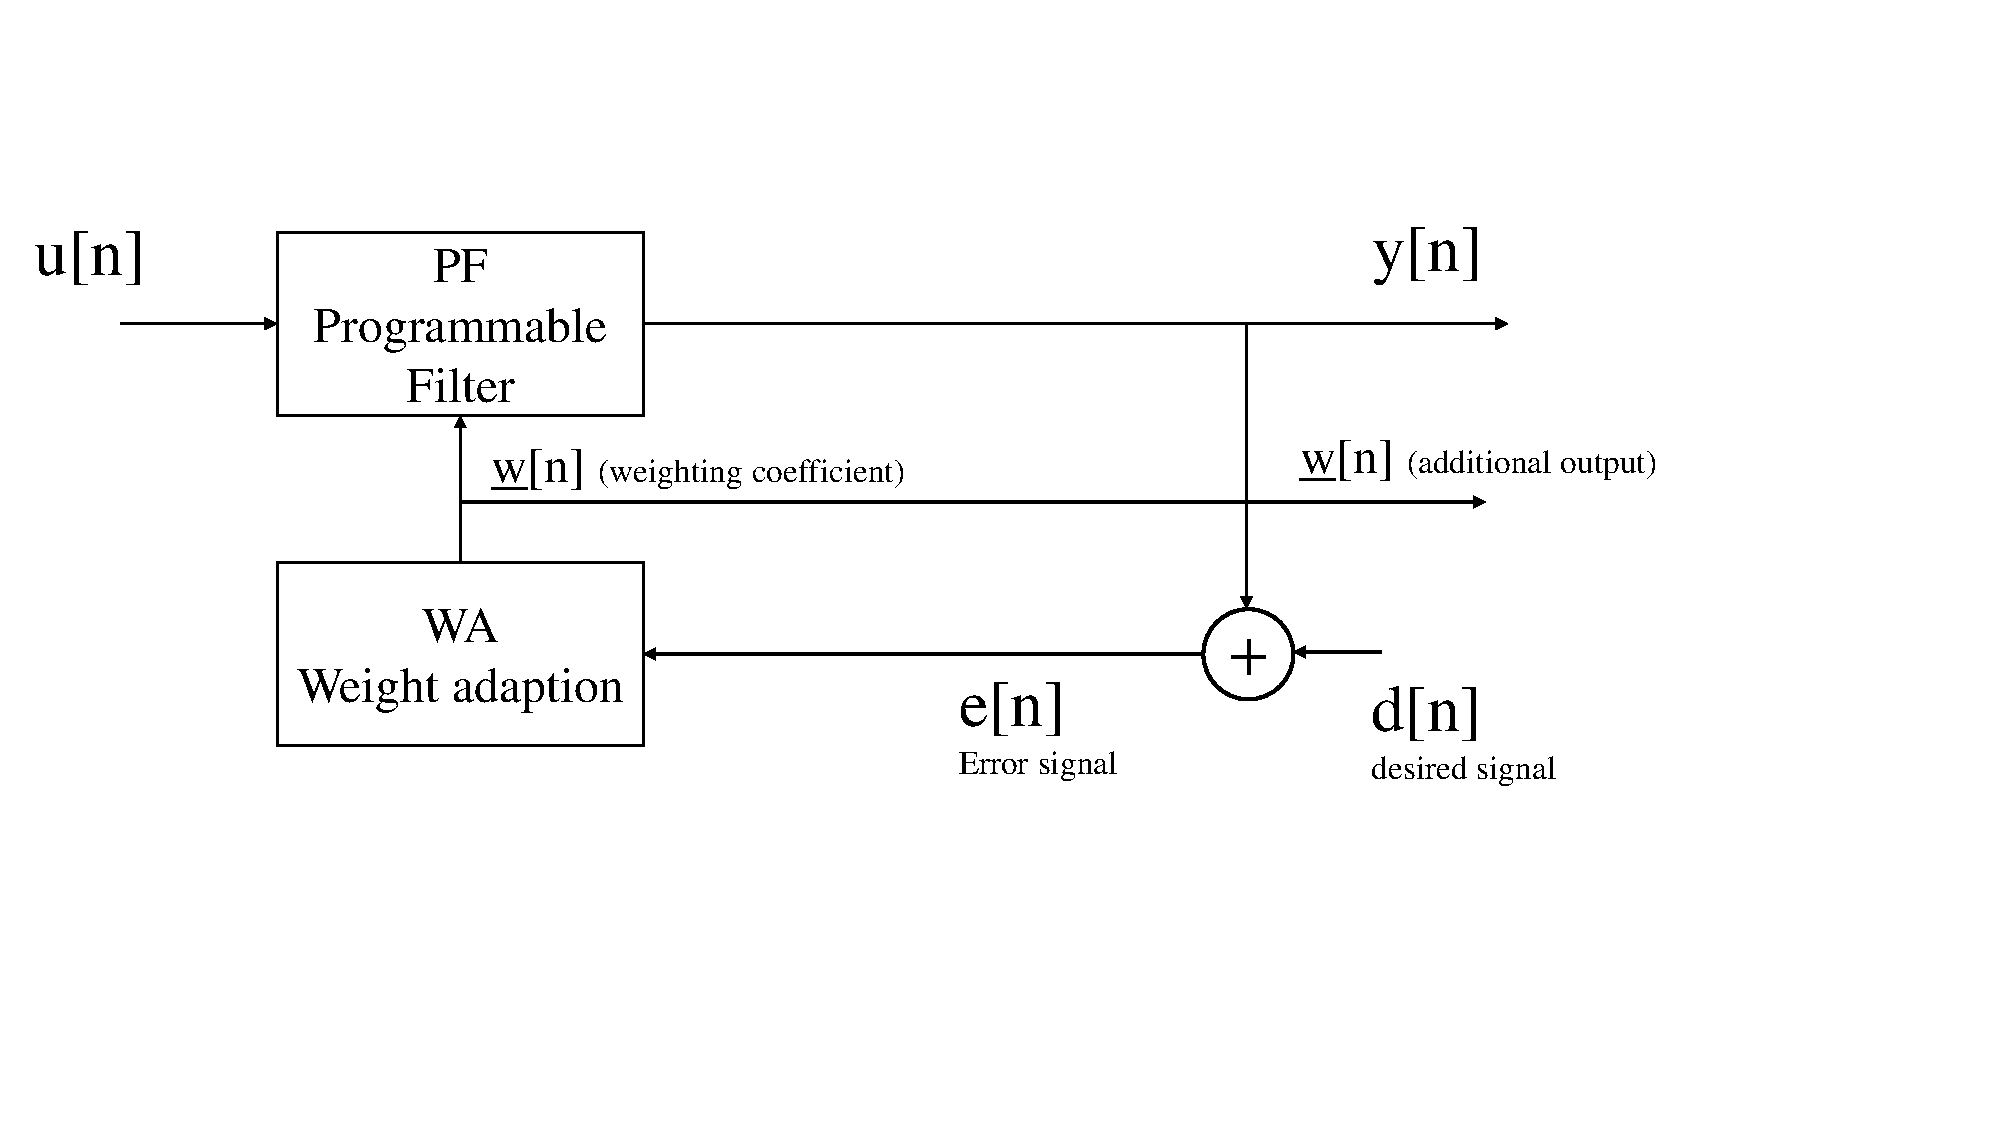
\includegraphics[scale=0.5, trim=0cm 5.5cm 0cm 3cm, clip]{adaptive_filter.pdf}
	\caption{Principle structure of an Adaptive Filter}
	\label{adaptive_filter} 
\end{figure}

$e[n] = 0 \pfeil \underline{w} [n+1] = \underline{w} [n]$
\subsubsection{The 4 Application Classes}
\textbf{System Identification}
	\begin{figure}[H]
		\centering
		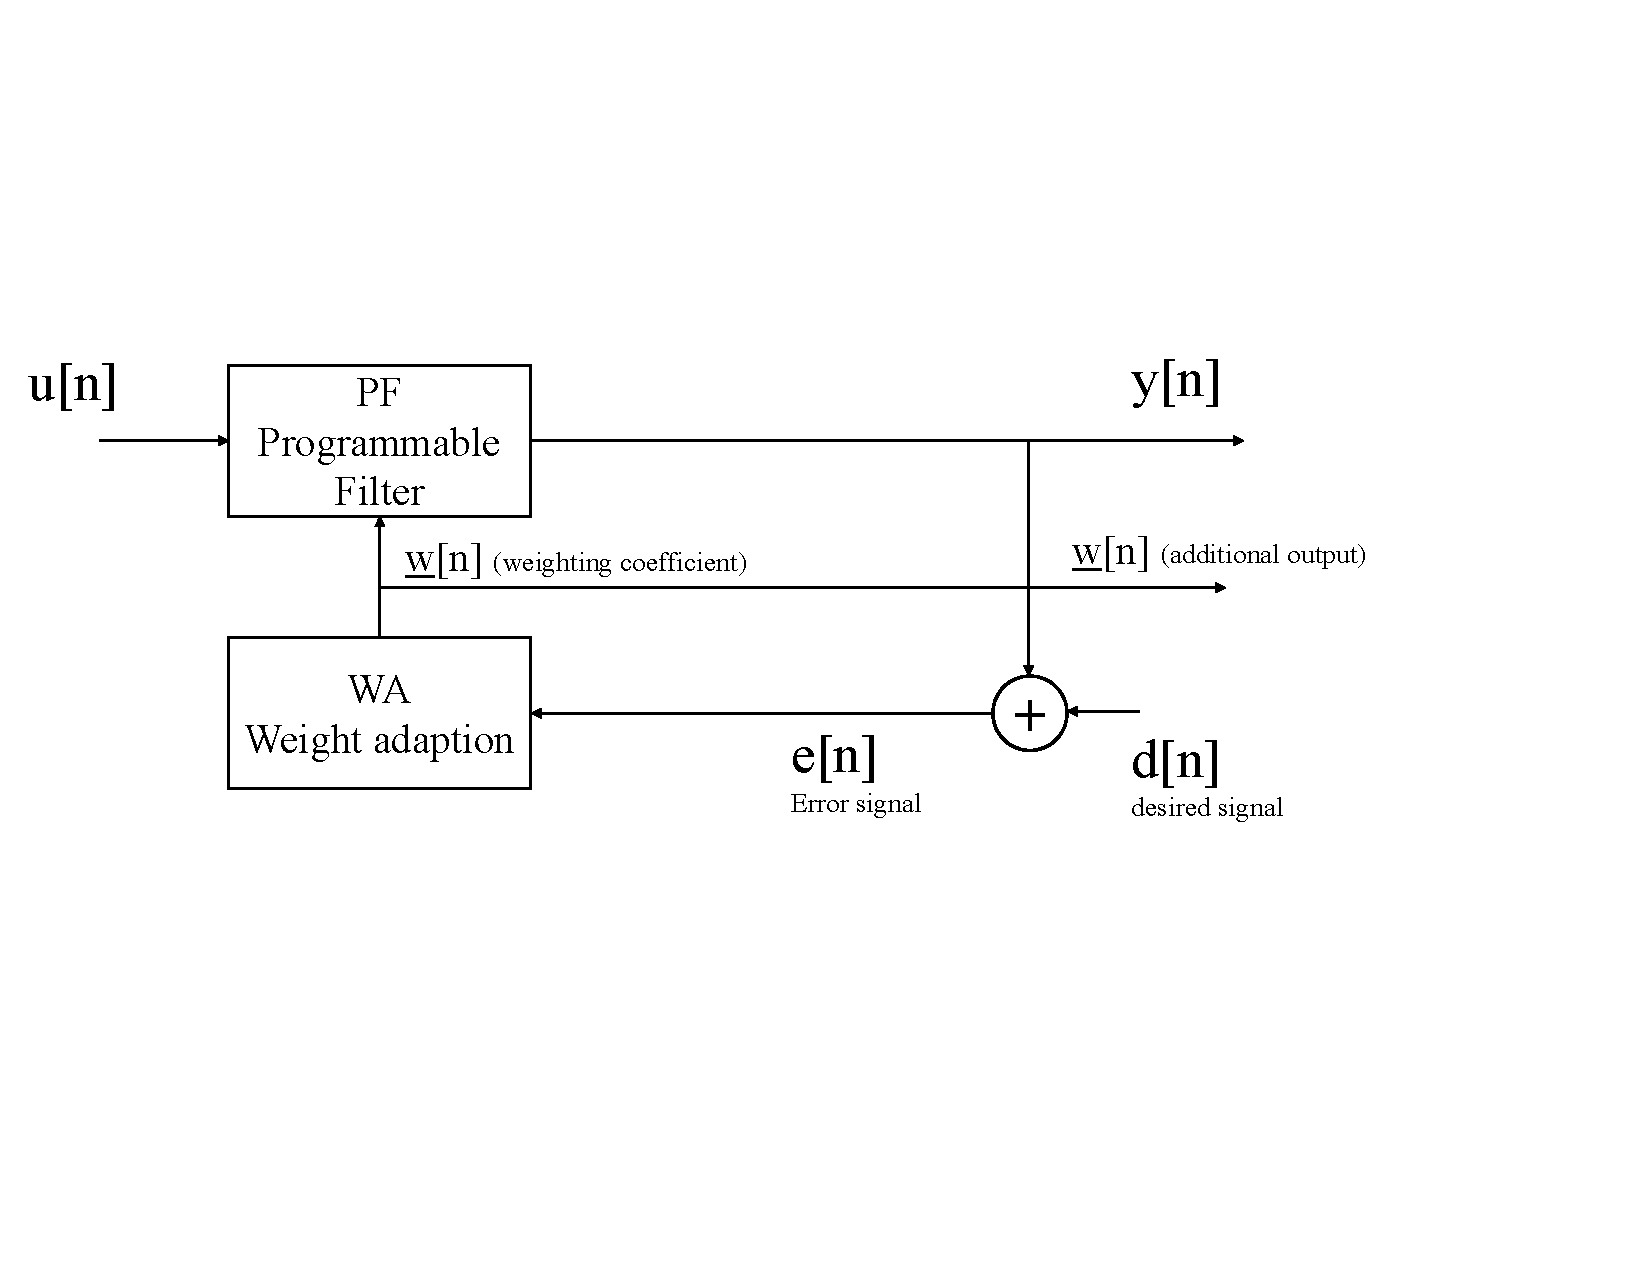
\includegraphics[scale=0.5, trim=0cm 5cm 0cm 5cm, clip]{system_identification.pdf}
		\caption{System identification}
		\label{system_identification} 
	\end{figure}

\textbf{Channel Estimation}
	\begin{figure}[H]
	\centering
	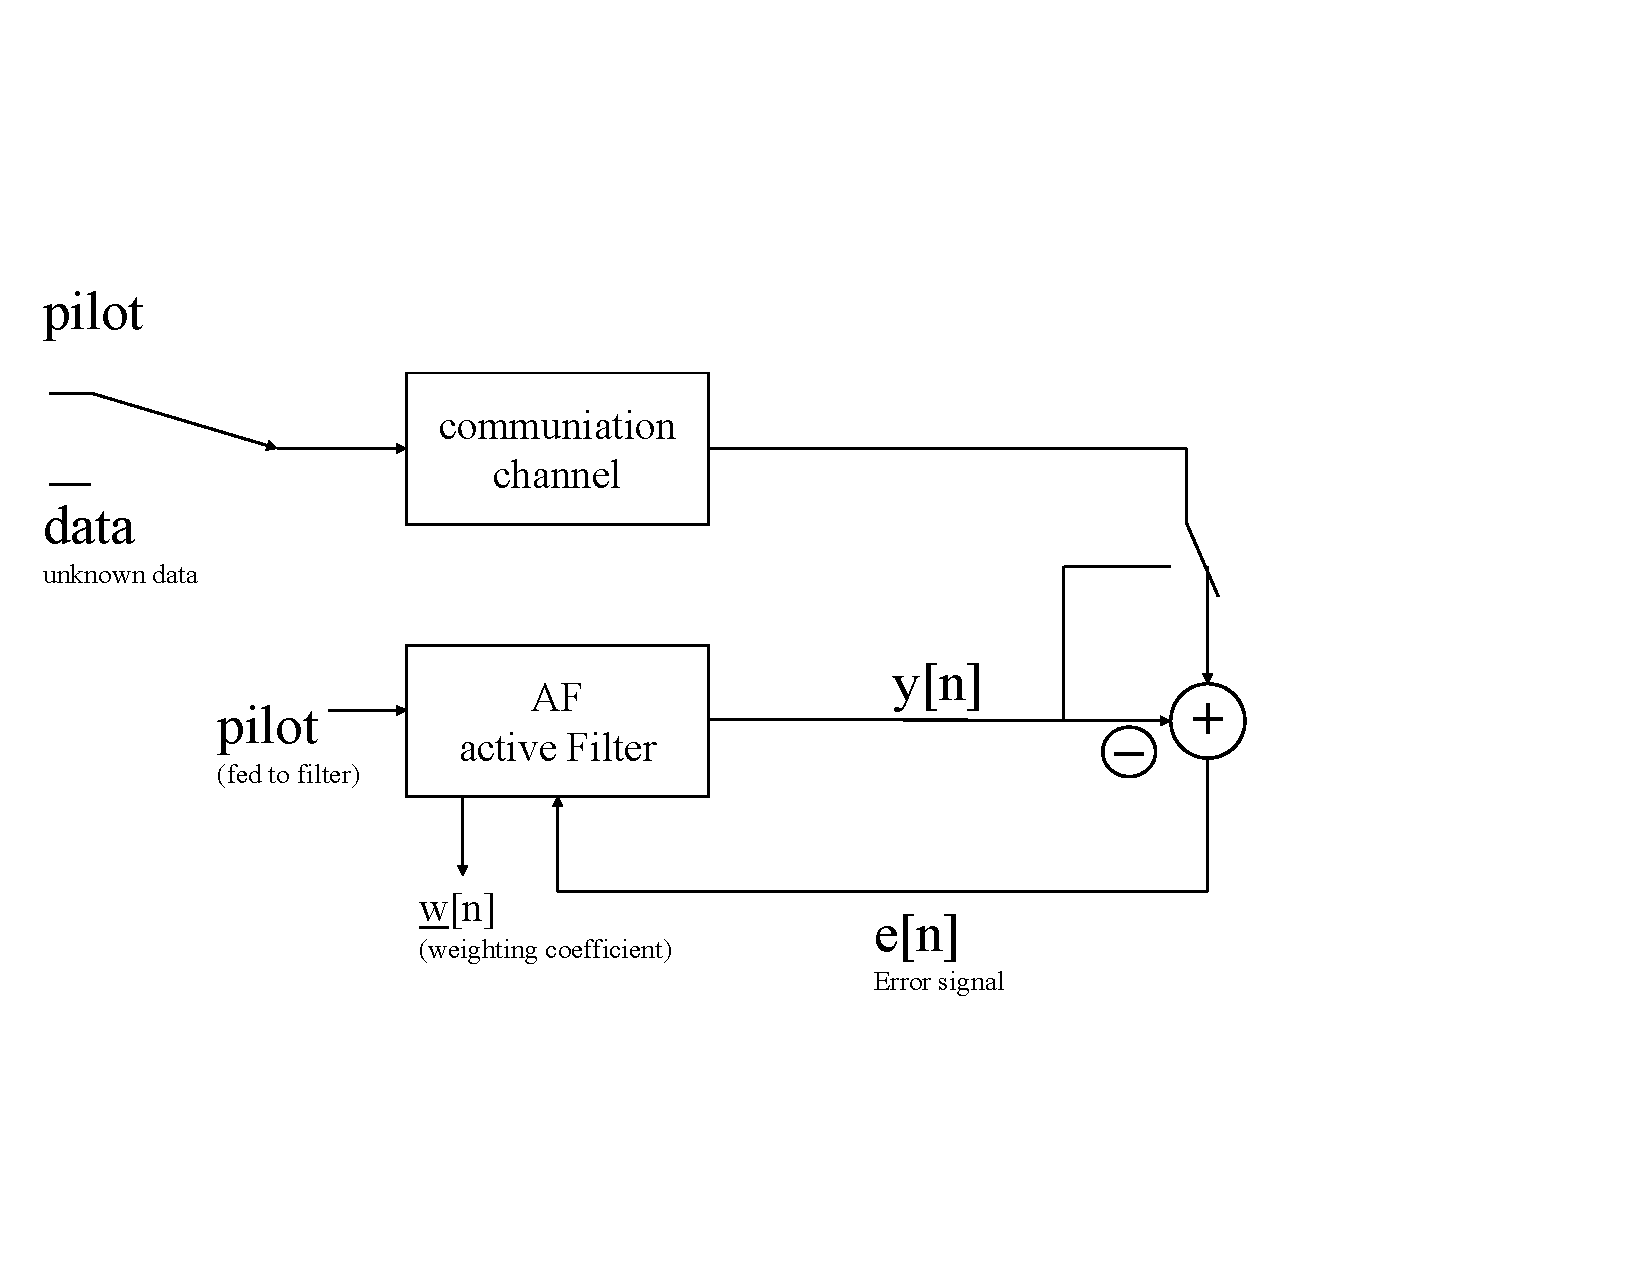
\includegraphics[scale=0.5, trim=0cm 4cm 0cm 5cm, clip]{channel_estimation.pdf}
	\caption{Channel Estimation}
	\label{channel_estimation} 
\end{figure}
The Pilot is a known data string. Either the transmitter and the receiver know the pilot. The data is unknown.

\textbf{Inverse Modelling}
	\begin{figure}[H]
	\centering
	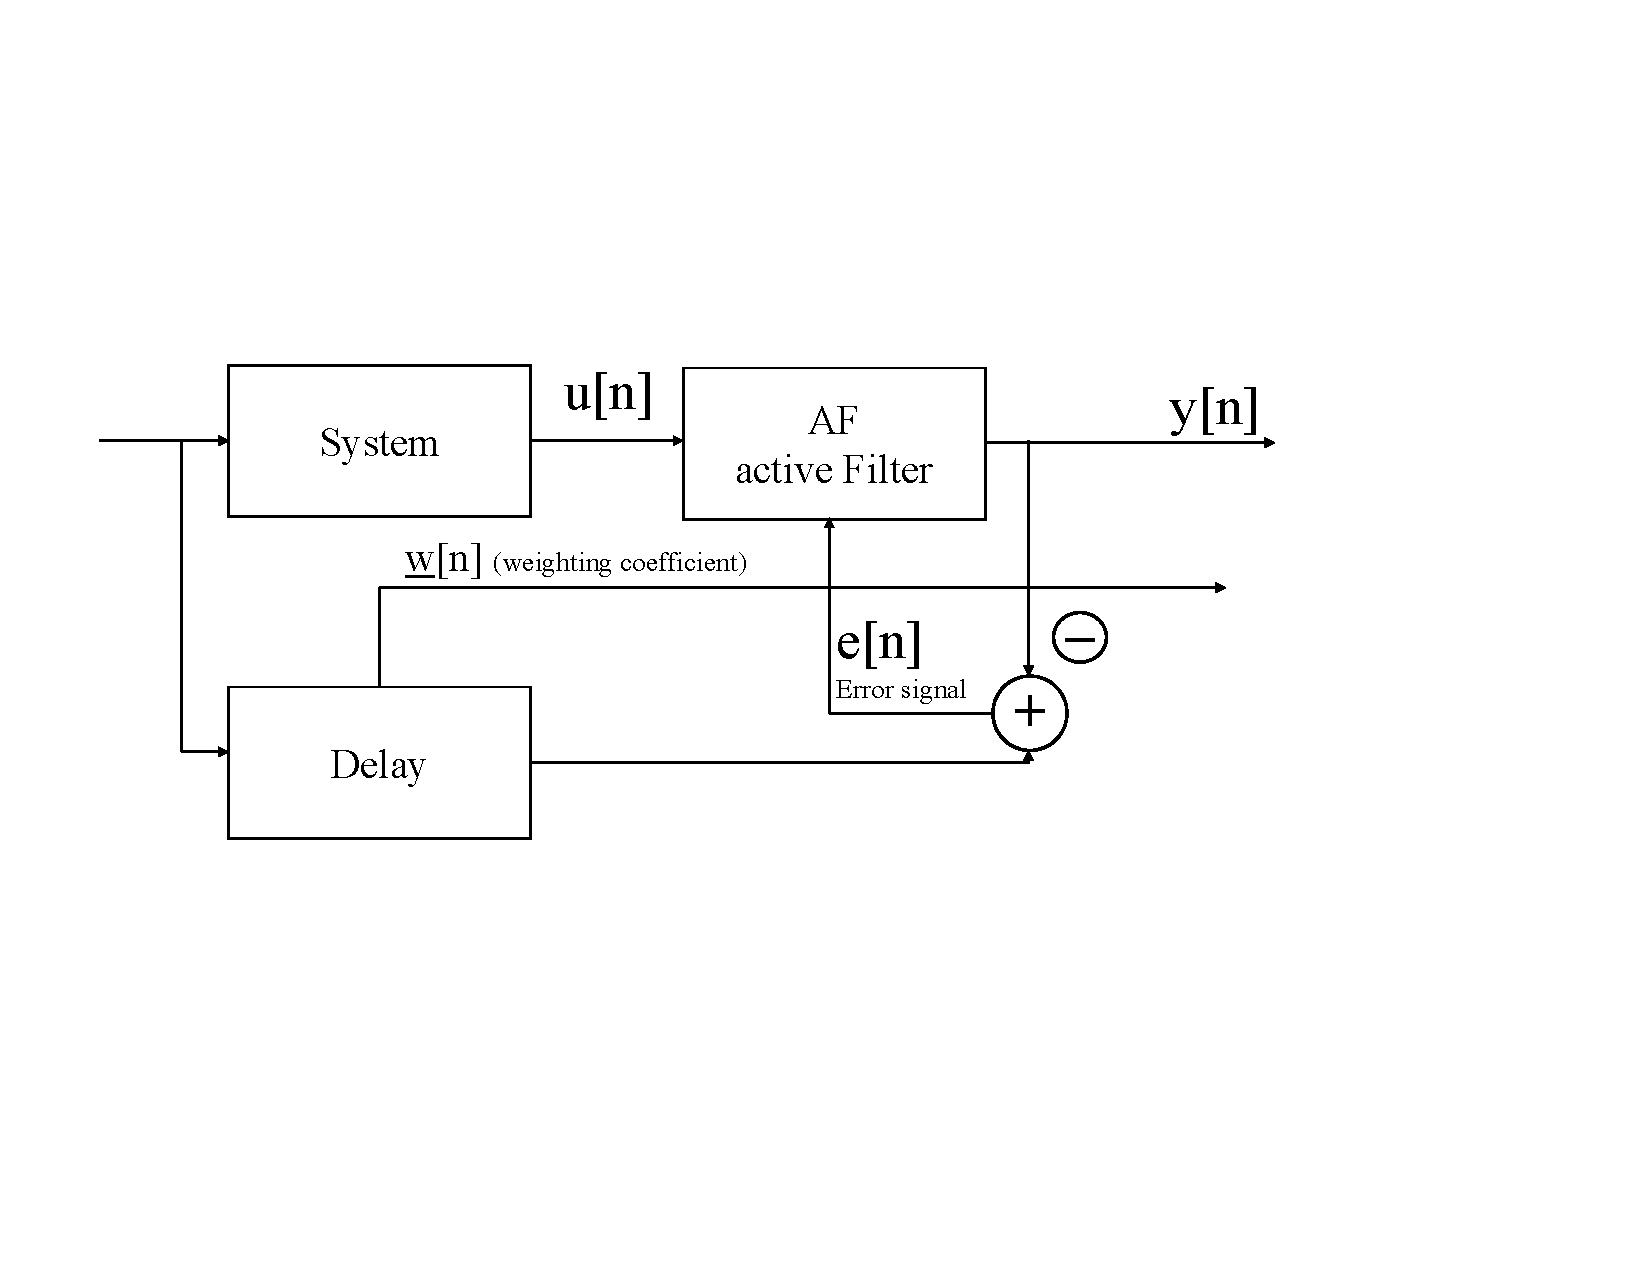
\includegraphics[scale=0.5, trim=0cm 7cm 0cm 5cm, clip]{inverse_modelling.pdf}
	\caption{Inverse Modelling}
	\label{inversemodelling} 
\end{figure}
Example to picture \ref{inversemodelling}: Channel equilization (interested in data, not the channel).\\
\textbf{Prediction}
	\begin{figure}[H]
	\centering
	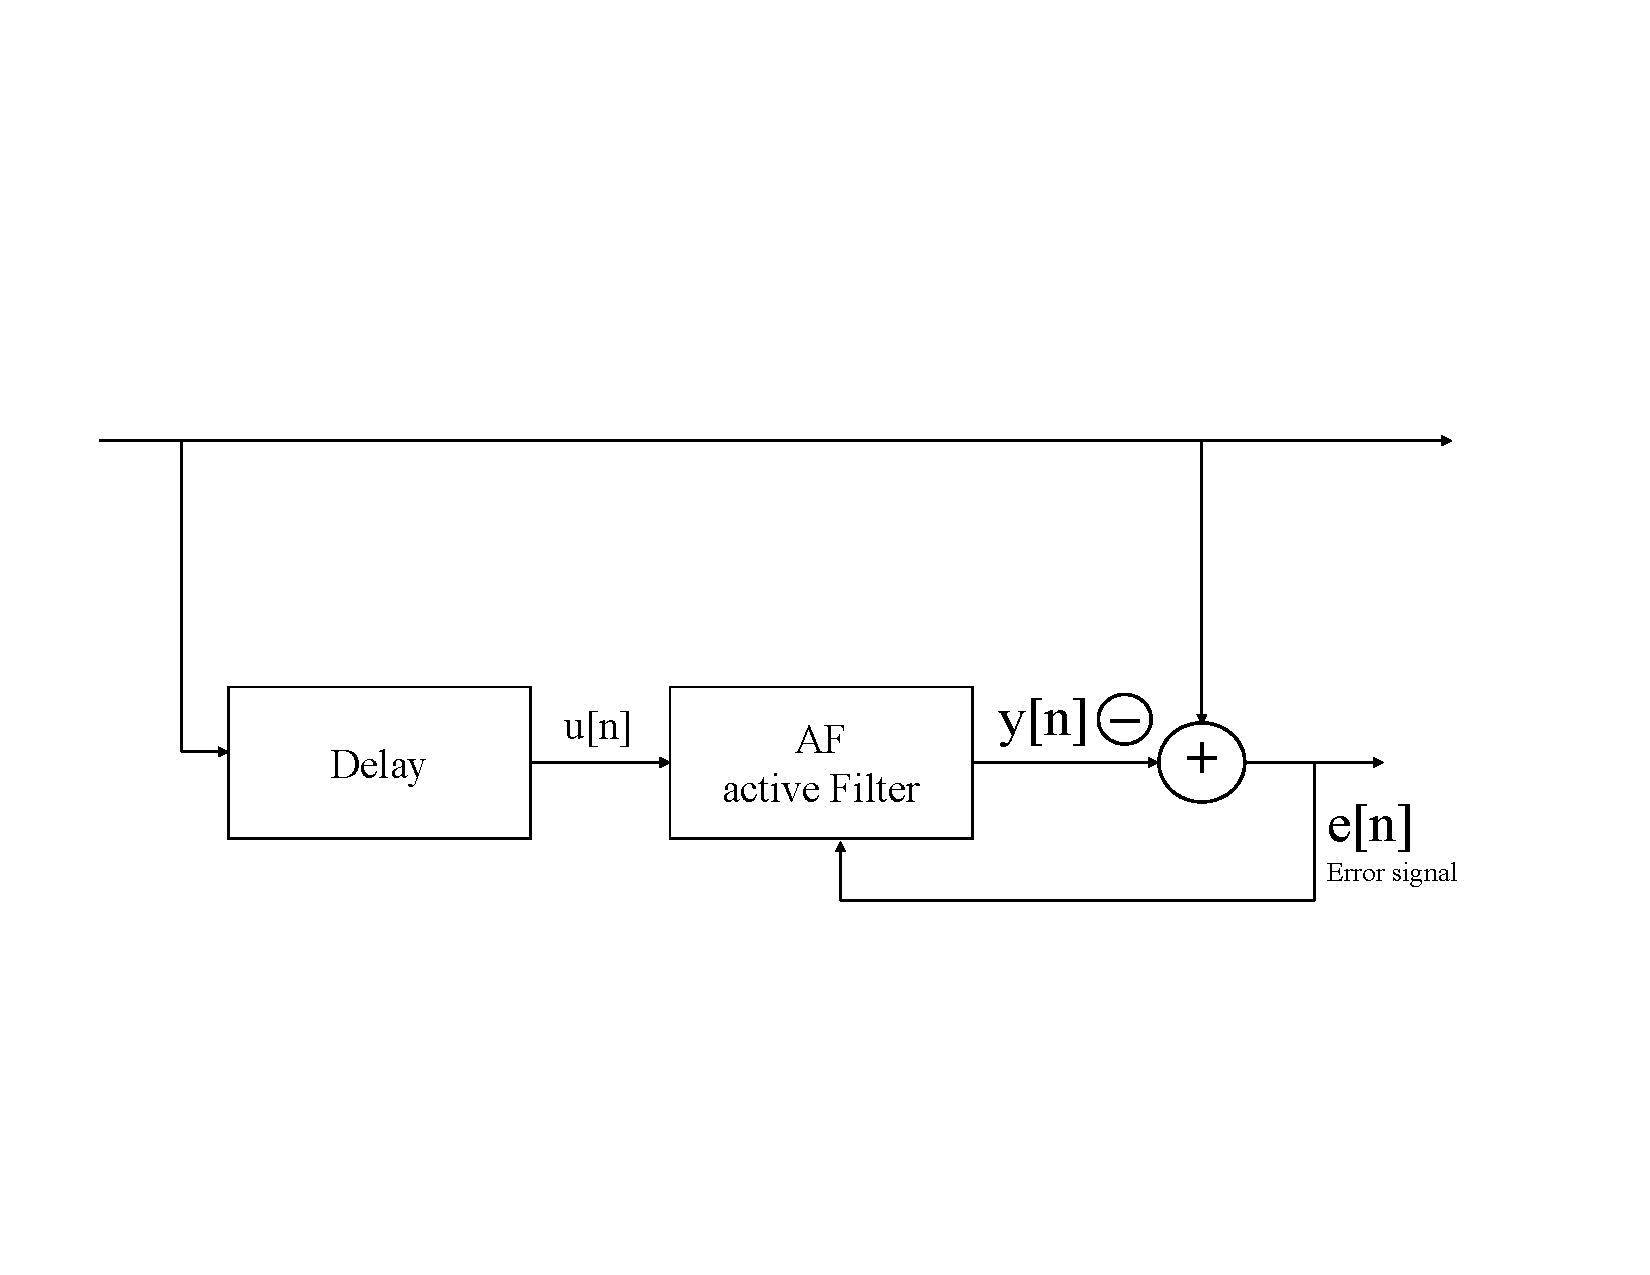
\includegraphics[scale=0.5, trim=0cm 4cm 0cm 5cm, clip]{prediction.pdf}
	\caption{Prediction}
	\label{prediction} 
\end{figure}
Notes to \ref{prediction}: Blind to future and present, but knows the past.. Trouble: if quantized e[n] won't work!\\
Therefore:\\
	\begin{figure}[H]
	\centering
	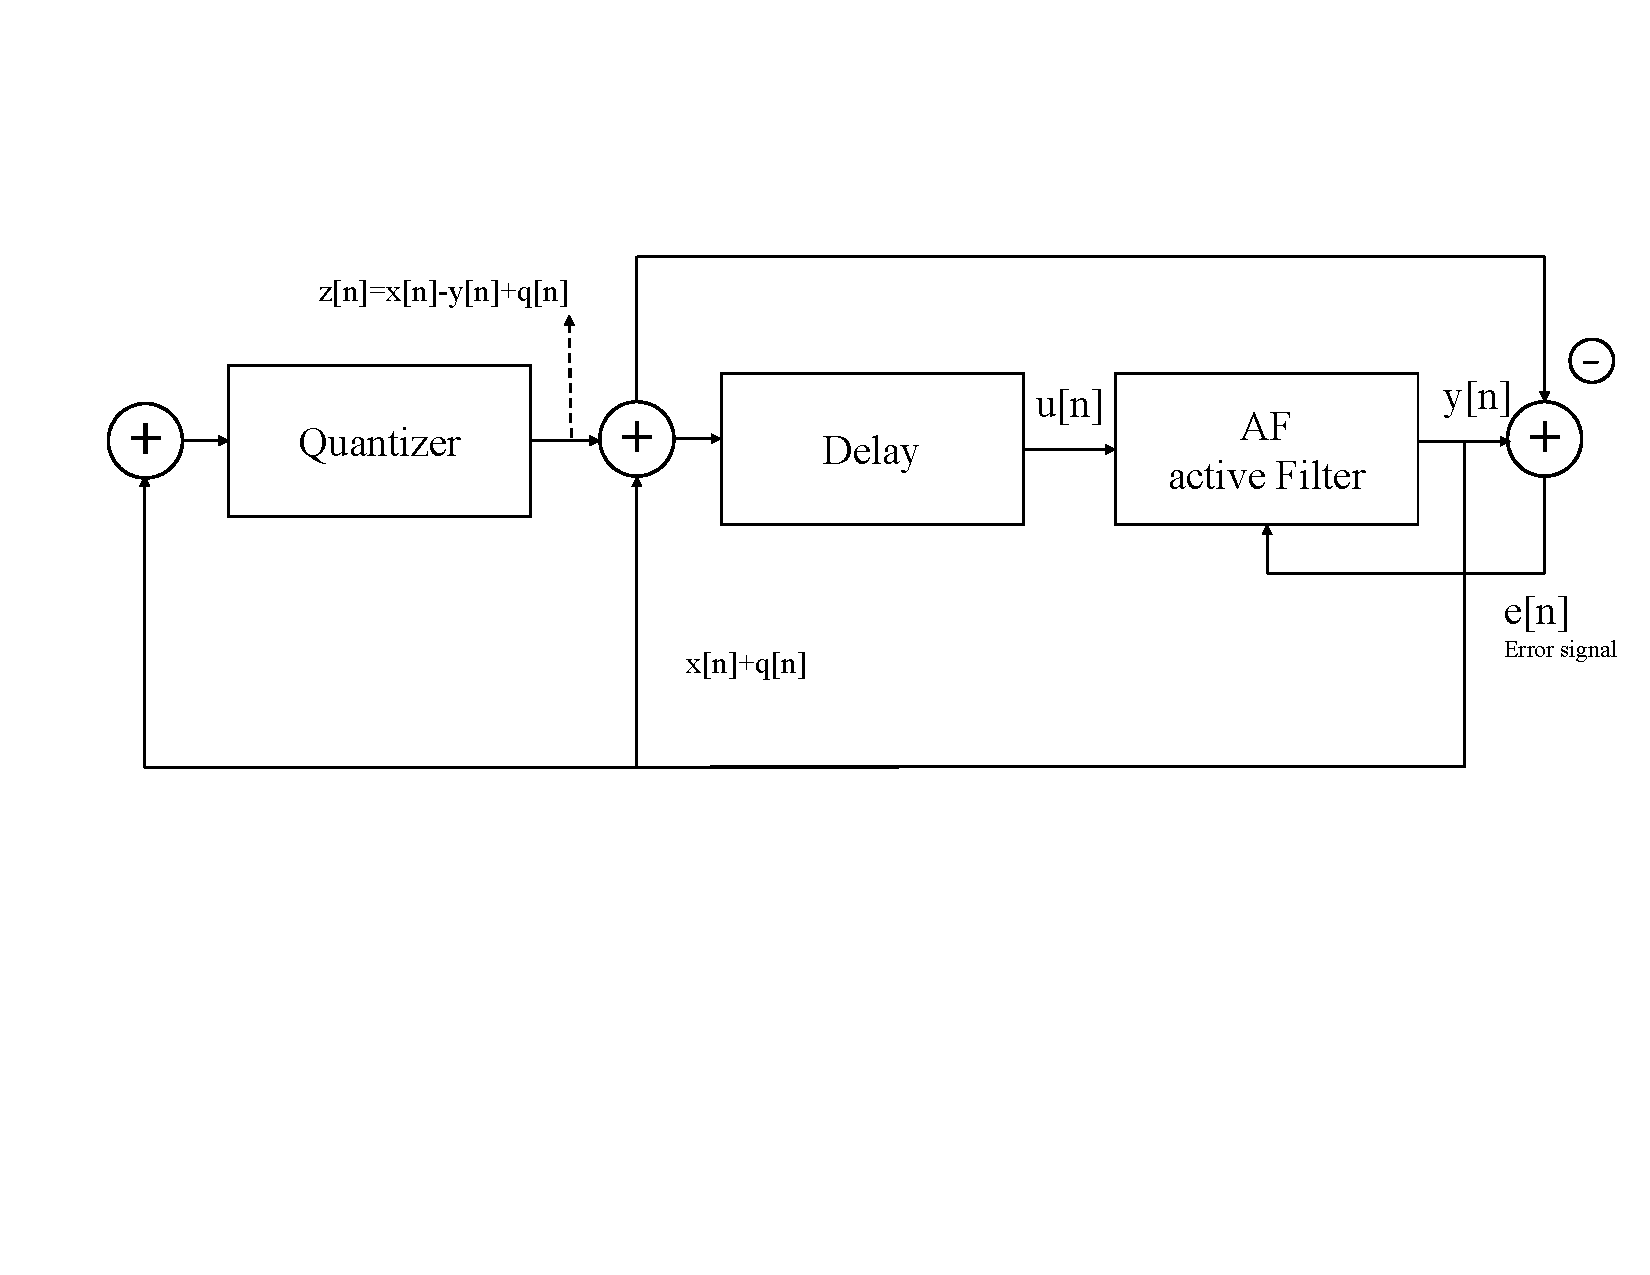
\includegraphics[scale=0.65, trim=0cm 7cm 0cm 3cm, clip]{compressor.pdf}
	\caption{Compressor}
	\label{compressor} 
\end{figure}
Predictive filter works well \pfeil if error is small\\
	\begin{figure}[H]
	\centering
	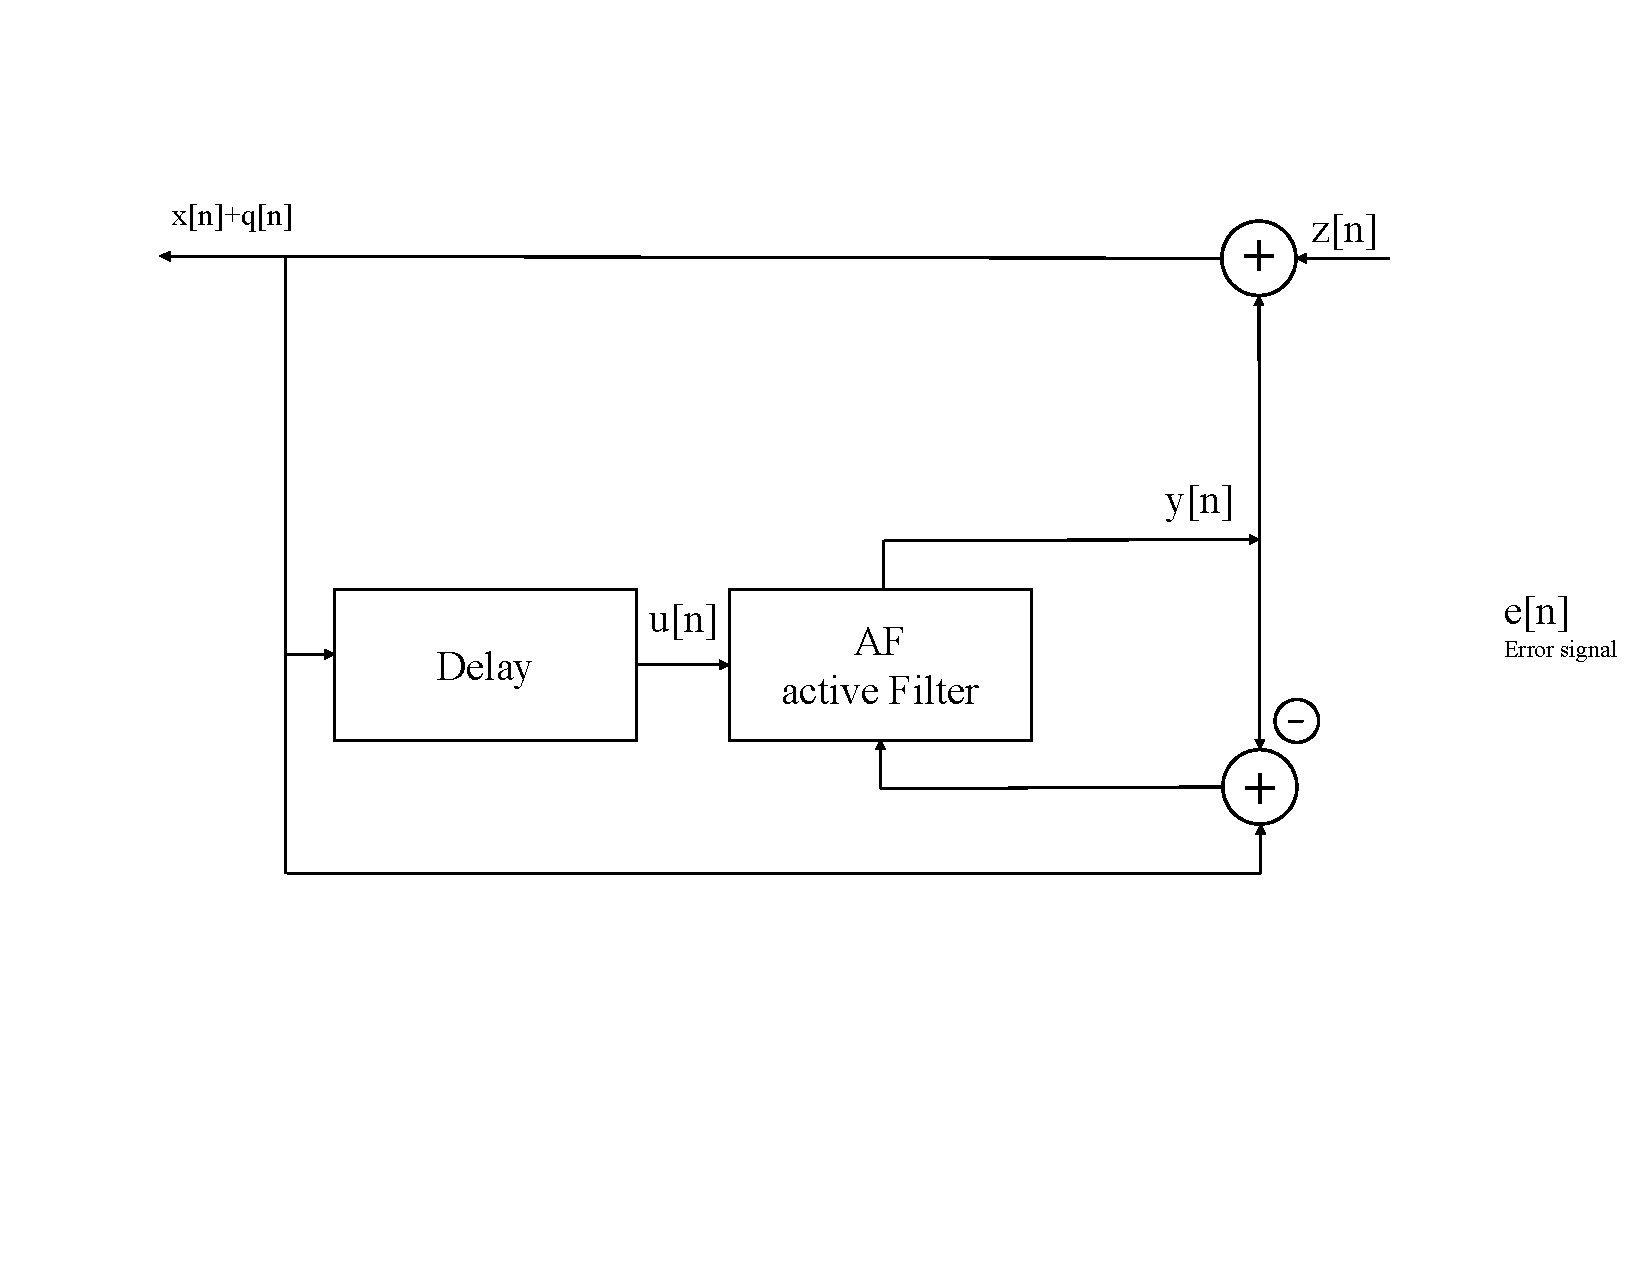
\includegraphics[scale=0.65, trim=0cm 5cm 0cm 2cm, clip]{decompressor.pdf}
	\caption{Decompressor}
	\label{decompressor} 
\end{figure}

\textbf{Interference Cancellation}
	\begin{figure}[H]
	\centering
	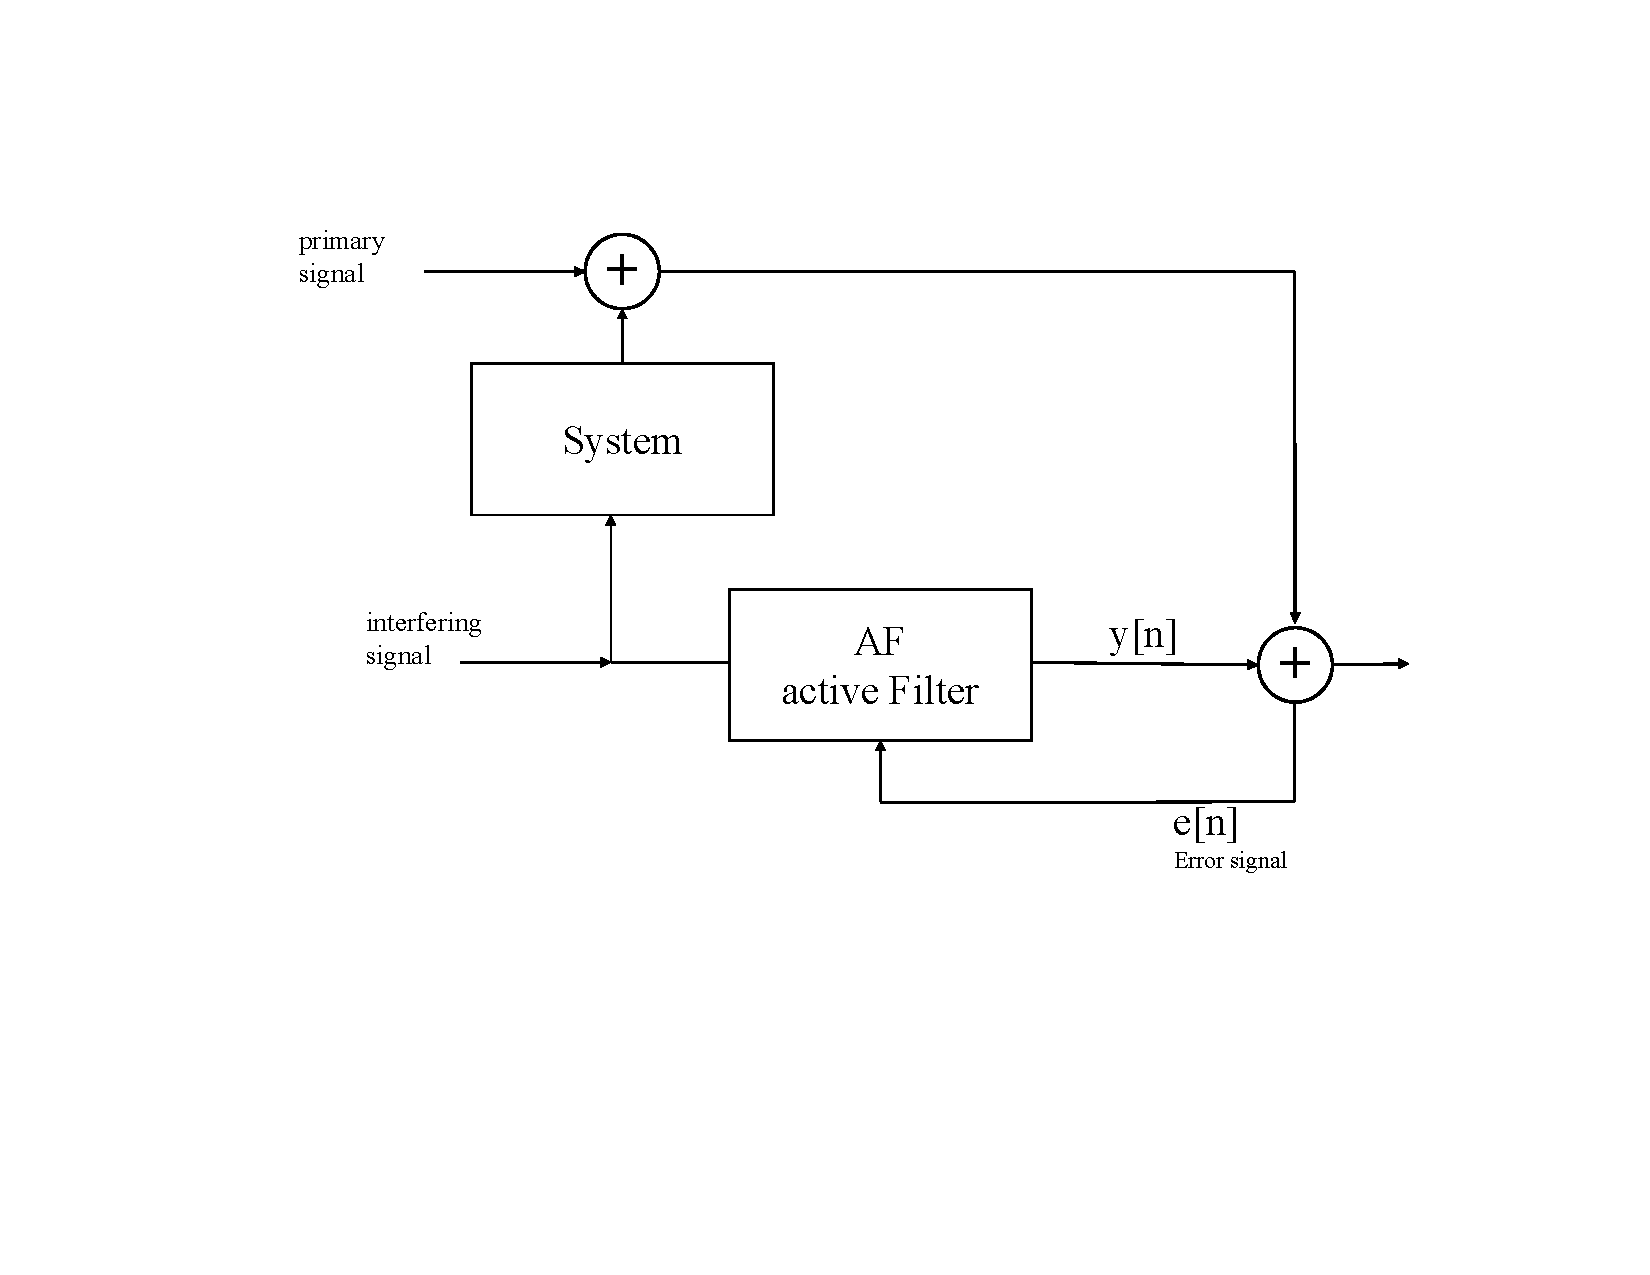
\includegraphics[scale=0.65, trim=0cm 6cm 0cm 3cm, clip]{interference_chanellation.pdf}
	\caption{Interference Cancellation}
	\label{interference1} 
\end{figure}
Assumption: The desired (primary) signal is statistically independent of the interfering signal.\\
For linear adaptive filters: uncorrelated is enough. 
\begin{figure}[H]
	\centering
	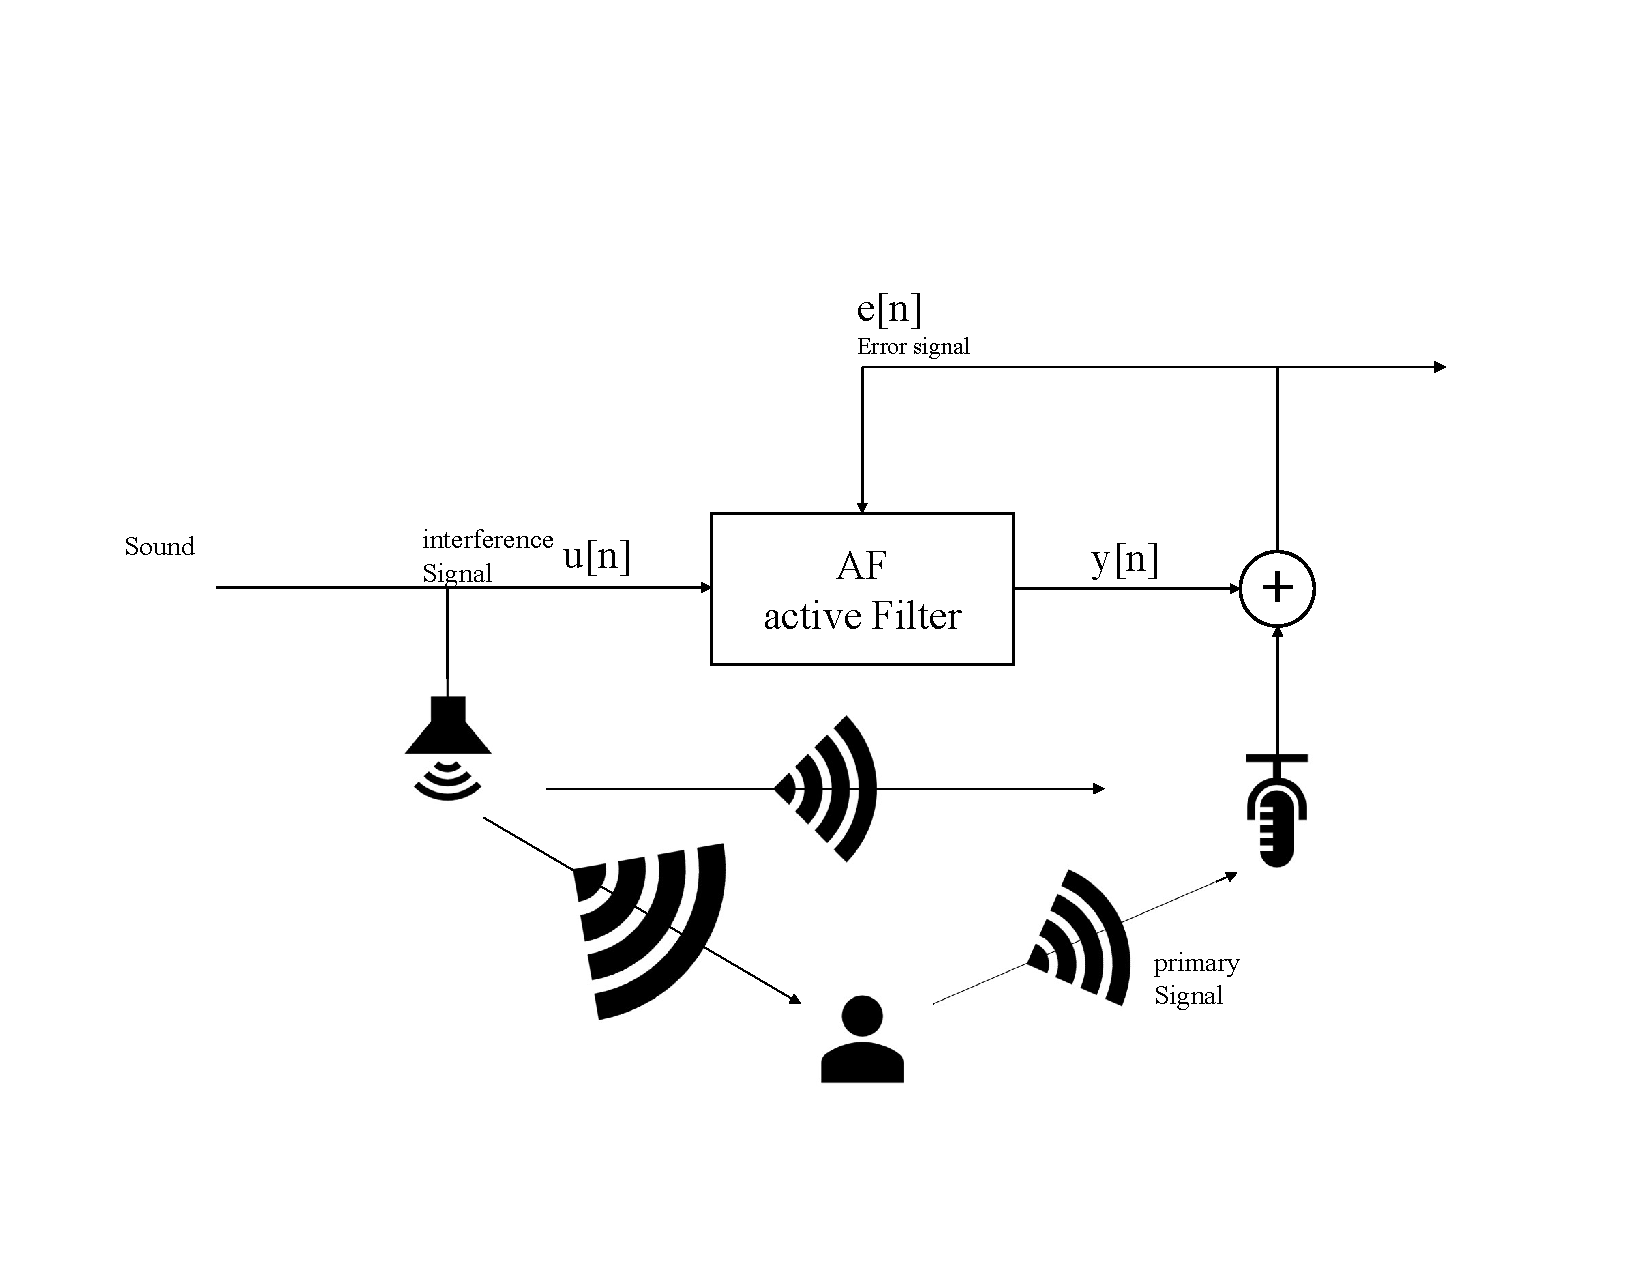
\includegraphics[scale=0.65, trim=0cm 3cm 0cm 4.5cm, clip]{interference_chanellation2.pdf}
	\caption{Example for an application for a an interference-cancelling-filter}
	\label{interference2} 
\end{figure}
For \ref{interference2}: Linear filters are better than nonlinear ones for this case. Filter tries to "'kill"' the interference because it knows, what has been played on the speaker.

\subsubsection{Complex Envelope}

\mybox{
\textbf{Definition:} 

$x(t)=\Re{u(t)e^{\j 2 \pi f_0 t}}$ 

with   
\begin{itemize}
\item $x(t)\in \mathbb{R}$: Real Signal
\item $u(t)\in \mathbb{R}$: Complex Envelope of $x(t)$
\item $f_0$: Center of Frequency; \quad $[f_0]=1 Hz$
\end{itemize}}

Notation with Magnitude and phase:

\quad $u(t)=|u(t)|\cdot e^{j\varphi_u(t)}$

Complex Envelope $u(t)$ mapped on signal $x(t)$ 

\quad $x(t)=\Re{u(t)e^{\j 2 \pi f_0 t}}=|u(t)|\cdot \cos (2\pi f_0 t + \varphi_u(t))=\frac{1}{2}u(t)\cdot e^{\j 2 \pi f_0 t}+\frac{1}{2}u^*(t)\cdot e^{-\j 2 \pi f_0 t}$

\with $\Re{z}=\frac{z+z^*}{2}$

approach to map signal $x(t)$ on complex envelope $u(t)\overset{?}{=}2x(t)\cdot e^{-j2 \pi f t }$  

\quad $2 x(t) \cdot e^{-j2 \pi f t } = 2 \Re{u(t)e^{\j 2 \pi f_0 t}}\cdot e^{-j2 \pi f t } =(u(t)e^{\j 2 \pi f_0 t} +u^*(t)e^{-\j 2 \pi f_0 t})\cdot e^{-j2 \pi f t }$

\quad $2 x(t) \cdot e^{-j2 \pi f t }  = u(t) + u^*(t)\cdot e^{-j4\pi f_0 t}$

Check approach with the Fourier transform:

$2 x(t) \cdot e^{-j2 \pi f t } \quad\laplace\quad U(f)+\int\limits_{-\infty}^{\infty}u^*(t)\cdot e^{-\j 4 \pi f_0 t}e^{\j 2 \pi f t}dt$


\with $\int\limits_{-\infty}^{\infty}u^*(t)\cdot e^{-\j 4 \pi f_0 t}e^{\j 2 \pi f t}dt 
=\int\limits_{-\infty}^{\infty}u^*(t)\cdot e^{-\j 2 \pi (f+2f_0) t}dt
=\left(\int\limits_{-\infty}^{\infty}u(t)\cdot e^{-\j 2 \pi (f+2f_0) t}\right)^*$

\qquad$=\left(\left.\underbrace{\int\limits_{-\infty}^{\infty}u(t)\cdot e^{-\j 2 \pi (f+2f_0) t}}_{U(f)}\right|_{-f-2f_0\to f }\right)^*=U^*(-f-2f_0)$

\pfeil $2 x(t) \cdot e^{-j2 \pi f t } \quad\laplace\quad U(f)+U^*(-f-2f_0)$

\begin{figure}[H]
	\centering
	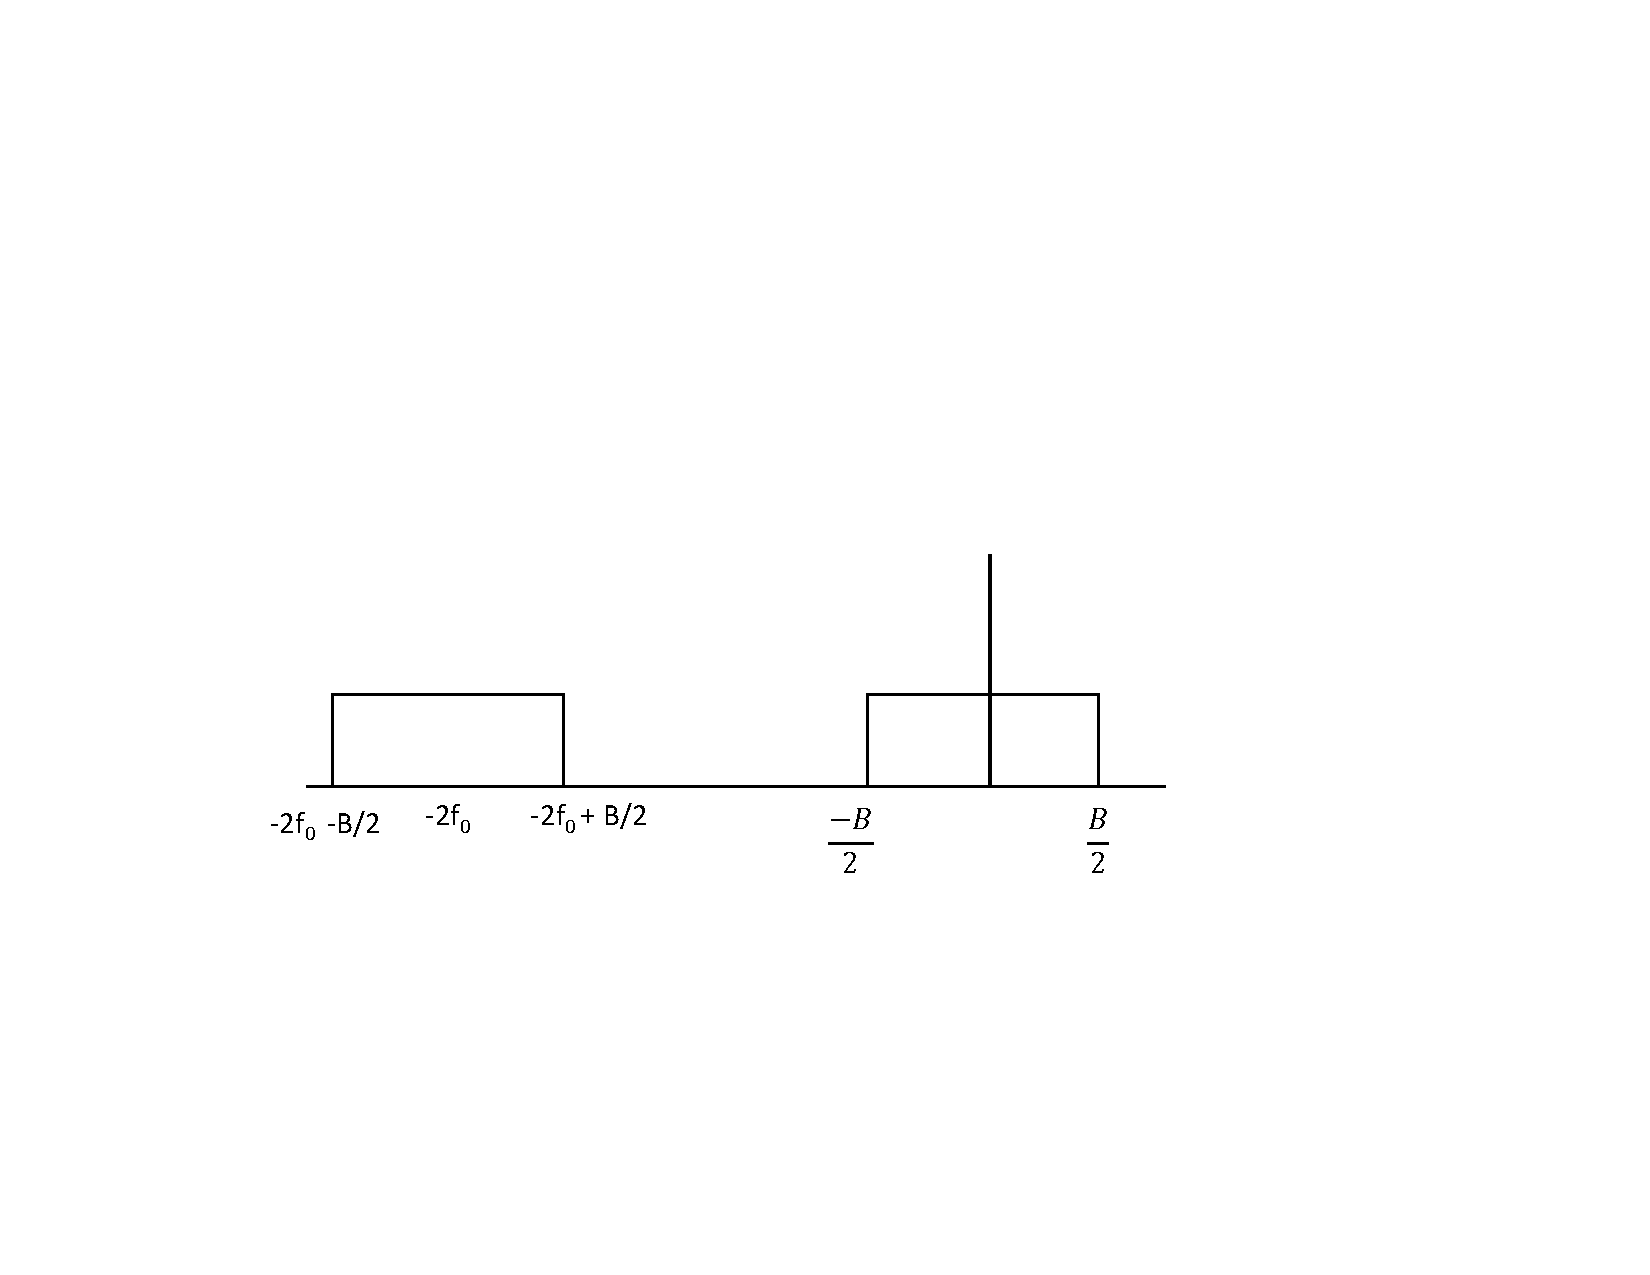
\includegraphics[scale=0.65, trim=0cm 6cm 0cm 11cm, clip]{bandlimitation.pdf}
	\caption{Result of the Fourier Transform}
	\label{ResultFourier} 
\end{figure}


\ \\
The result shows an additional shifted envelope \pfeil therefore a low pass filter (LPF) is needed to suppress overlapping (aliasing).\pfeil band limitation\\
\pfeil $u(t) = LPF( x(t) \cdot 2\cdot e^{-j2 \pi f t } )$
\ \\$x(t) \iff u(t)$ $[$It's not a Fourier transform, but related.$]$\\

\textbf{Constraints for Bandwidth:}

Out of Picture \ref{ResultFourier}:

\quad $-2f_0+\frac{B}{2} \leq -\frac{B}{2} $ 

\mybox{
\pfeil  $B \leq 2 f_0$ \qquad or \qquad $f_0 \geq \frac{B}{2}$}


\begin{figure}[H]
	\centering
	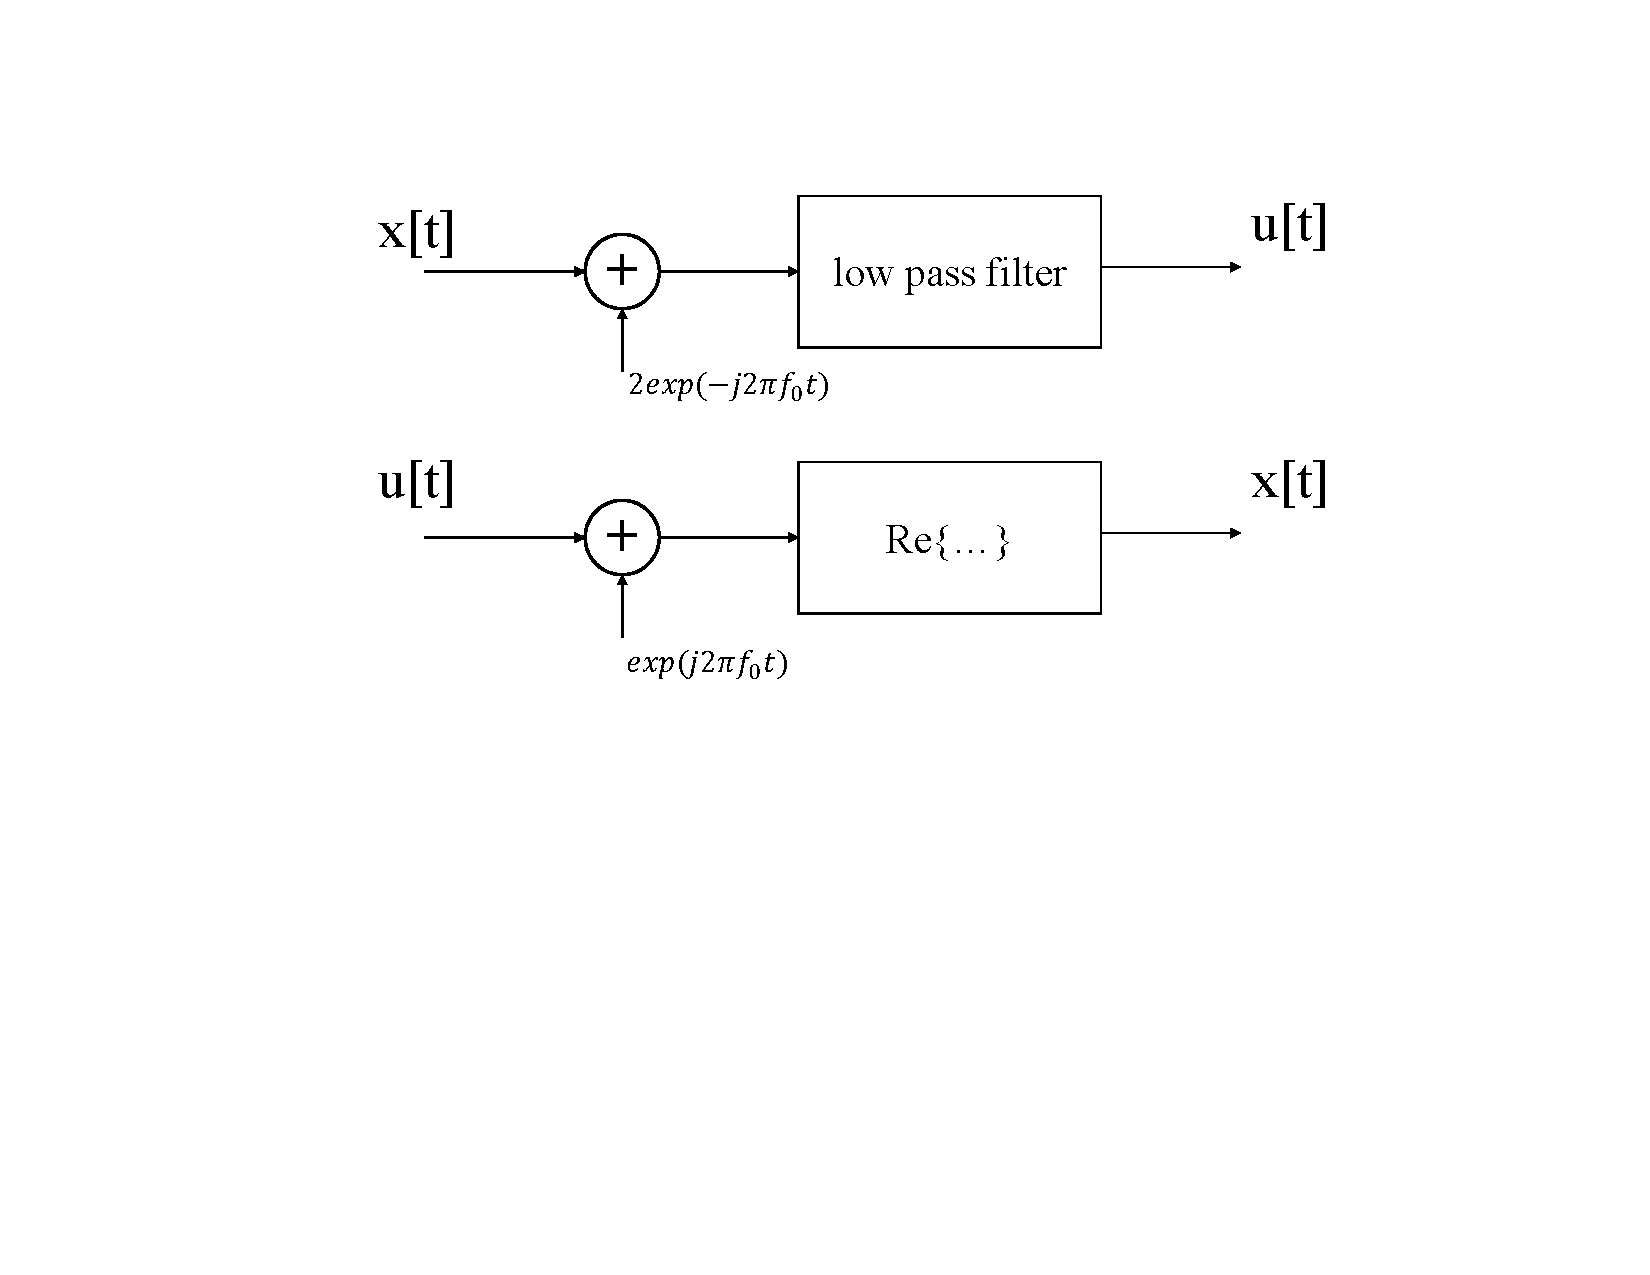
\includegraphics[scale=0.65, trim=0cm 10cm 0cm 3cm, clip]{bandpass_not_overlapping.pdf}
	\caption{Transformation from complex envelope and signal as block diagram and vice versa}
	\label{complexEnvelopTransform} 
\end{figure}
$x(t) \iff u(t)$ $[$It's not a fourier transform, but related.$]$\\
\ \\

\subsubsection{Whatever we did here - No. 264}
\paragraph{\texorpdfstring{Ivrla\v c}{Ivrlac} the dimensions Conqueror }

\[\sum_{m}\underbrace{a_m}_{\in \mathbb{R}}x(t-t_m) \iff \sum_{m}\underbrace{a_m \cdot e^{-i 2\pi f_0 t_m}}_{b_m \in \mathbb{C}}u(t-t_m)  = \sum_{m} |b_m| \cdot e^{j\varphi_m} u(t-t_m)\] \\
Under condition of:$\vert b_m\vert = a_m \quad  \varphi_{b_m}= -2\pi f_0 t_m$\\
Note: Correspondence is linear; center frequency has to be known.\\

\begin{doublespace} 
$u(t) \iff x(t) = \Re { u(t) e^{j2\pi f_0 t} }$\\
\paragraph{Approach - Complex Envelope shifted and scaled to fit a real signal}\ \\
$w^* u(t-\tau) \ct c\cdot x(t-\overset{\sim}{t}) = x'(t) \with c \in \mathbb{R}$



$\underbrace{w^*}_{const.}\cdot u(t-\tau)$  $\ct x'(t)= \Re {w^*\cdot u(t-\tau) e^{j2\pi f_0 t}},\\ \with \quad u(t)= |u(t)| e^{j2\pi f_0 (t-\tau)} \quad w=|w|e^{j\varphi_w}$\\


$c\cdot x(t-\tau)= \Re{w^* u(t-\tau e^{j2\pi f_0 t})}$

$c\cdot \Re{u(t-\overset{\sim}{t})\cdot e^{j2\pi f_0(t-\overset{\sim}{t})}}  = \Re{w^*\cdot u(t-\tau)\cdot e^{j2\pi f_0 t}} $\\
$c \cdot |u(t-\overset{\sim}{t})|\cos(2\pi f_0t-2\pi f_0 \overset{\sim}{t} + \varphi_u(t-\overset{\sim}{t})) = |w||u(t-\tau)|\cos(2\pi f_0 t + 2\pi \varphi_u (t-\tau)-\varphi_w)$\\
\pfeil cos(arg) should be equal!\\
$2\pi f_0t-2\pi f_0 \overset{\sim}{t} + \varphi_u(t-\overset{\sim}{t}) = 2\pi f_0 t + 2\pi \varphi_u (t-\tau)-\varphi_w$\\
$2\pi f_0t-2\pi f_0 \overset{\sim}{t} + \varphi_u(t-\overset{\sim}{t}) = 2\pi f_0 t + 2\pi \varphi_u (t-\tau)-\varphi_w+ q\cdot2\pi \with q \in \mathbb{Z}$\\
$f_0 \tilde{t}=\frac{\varphi_u(t-\tilde{t})-\varphi_u(t-\tau)+\varphi_w}{2\pi}-q$\\
Non-linear in $\tilde{t}$\\
Substitution: $\tilde{t}=\tau+\Delta t$ \\
$f_0 \Delta t=\frac{\varphi_u(t-\overset{\sim}{t}-\Delta t)-\varphi_u(t-\tau)+\varphi_w}{2\pi}-f_0\tau-q$\\
\textbf{Choose} q:\\
$0\leq f_0 \Delta t <1$\\
\begin{tabular}{ll}
\textbf{Assumption}: & u(t) is \textbf{narrow band}\\ 
 &$u(t-t')\approx u(t)$ \with $|t'|\leq \frac{1}{f_0}$\\
 &$f_0 \Delta t = (\frac{\varphi_w}{2\pi}-f_0\tau)mod(1)$\\
 &$\Delta t= (\frac{\varphi_w}{2\pi f_0}-\tau)mod(\frac{1}{f_0})$\\
\end{tabular}\\

\mybox{
$\tilde{t}= (\frac{\varphi_w}{2\pi f_0}-\tau)mod(\frac{1}{f_0})+\tau$\\
$c=|w|$ Complex envelope only for narrow band!}
\ \\


\paragraph{Power computation}\ \\ 
\quad $x(t)=\frac{1}{2}u(t)\cdot e^{\j 2 \pi f_0 t}+\frac{1}{2}u^*(t)\cdot e^{-\j 2 \pi f_0 t} \quad |(\bullet)^2$\\
\quad $x(t)^2=(\frac{1}{2}u(t)\cdot e^{\j 2 \pi f_0 t}+\frac{1}{2}u^*(t)\cdot e^{-\j 2 \pi f_0 t})(\frac{1}{2}u(t)\cdot e^{\j 2 \pi f_0 t}+\frac{1}{2}u^*(t)\cdot e^{-\j 2 \pi f_0 t})$\\
\quad $x(t)^2=\frac{1}{4}u^2(t)\cdot e^{\j 4 \pi f_0 t}
+\frac{1}{2}u(t)\cdot u^*(t)+
\frac{1}{4}u^{2*}(t)\cdot e^{-\j 4 \pi f_0 t}$\\
\with $\frac{1}{2}u(t)\cdot u^*(t)=\frac{1}{2}|u(t)|^2 $\\
$ \with \frac{1}{4}u^2(t)\cdot e^{\j 4 \pi f_0 t}+\frac{1}{4}u^{2*}(t)\cdot e^{-\j 4 \pi f_0 t}=\frac{1}{4}u^2(t)\cdot e^{\j 4 \pi f_0 t}+(\frac{1}{4}u^{2}(t)\cdot e^{\j 4 \pi f_0 t})^*=\frac{1}{2}\Re{u^2(t)e^{j4\pi f_0t}}$\\
Square of Magnitude\\
$|x(t)|^2= \frac{1}{2}|u(t)|^2 + \frac{1}{2}\Re{u^2(t)e^{j4\pi f_0t}}$\\
Get Time average with expectation:\\
Restrict u(t) to be proper:\\
$E[u^2(t)]=0$\\ $E[|x(t)|^2]=\frac{1}{2}E[|u(t)|^2]$\\
$u(t)= a(t)+jb(t)$\\
$u^2(t)= a^2(t) + 2j a(t)b(t) -b^2(t)$\\
$E[u^2]= \underbrace{E[a^2(t)-b^2(t)]}_{=0}+\underbrace{2jE[a(t)b(t)]}_{=0}\overset{!}{=}0$ \quad (widely linear processing)\\
\textbf{Mean Time square average for narrow band:}  (equals power)\\
$\overline{x^2(t)}=f_0 \cdot\int\limits_{t-\frac{1}{2f_0}}^{t+\frac{1}{2f_0}}x^2(\tau) d\tau \approx \frac{1}{2}|u(t)|^2 $\\
time average $x^2$ is a good assumption. \pfeil We will stick with narrow band assumption \pfeil both will work.\\
\end{doublespace}

\subsubsection{FIR-Filter}
\begin{figure}[H]
	\centering
	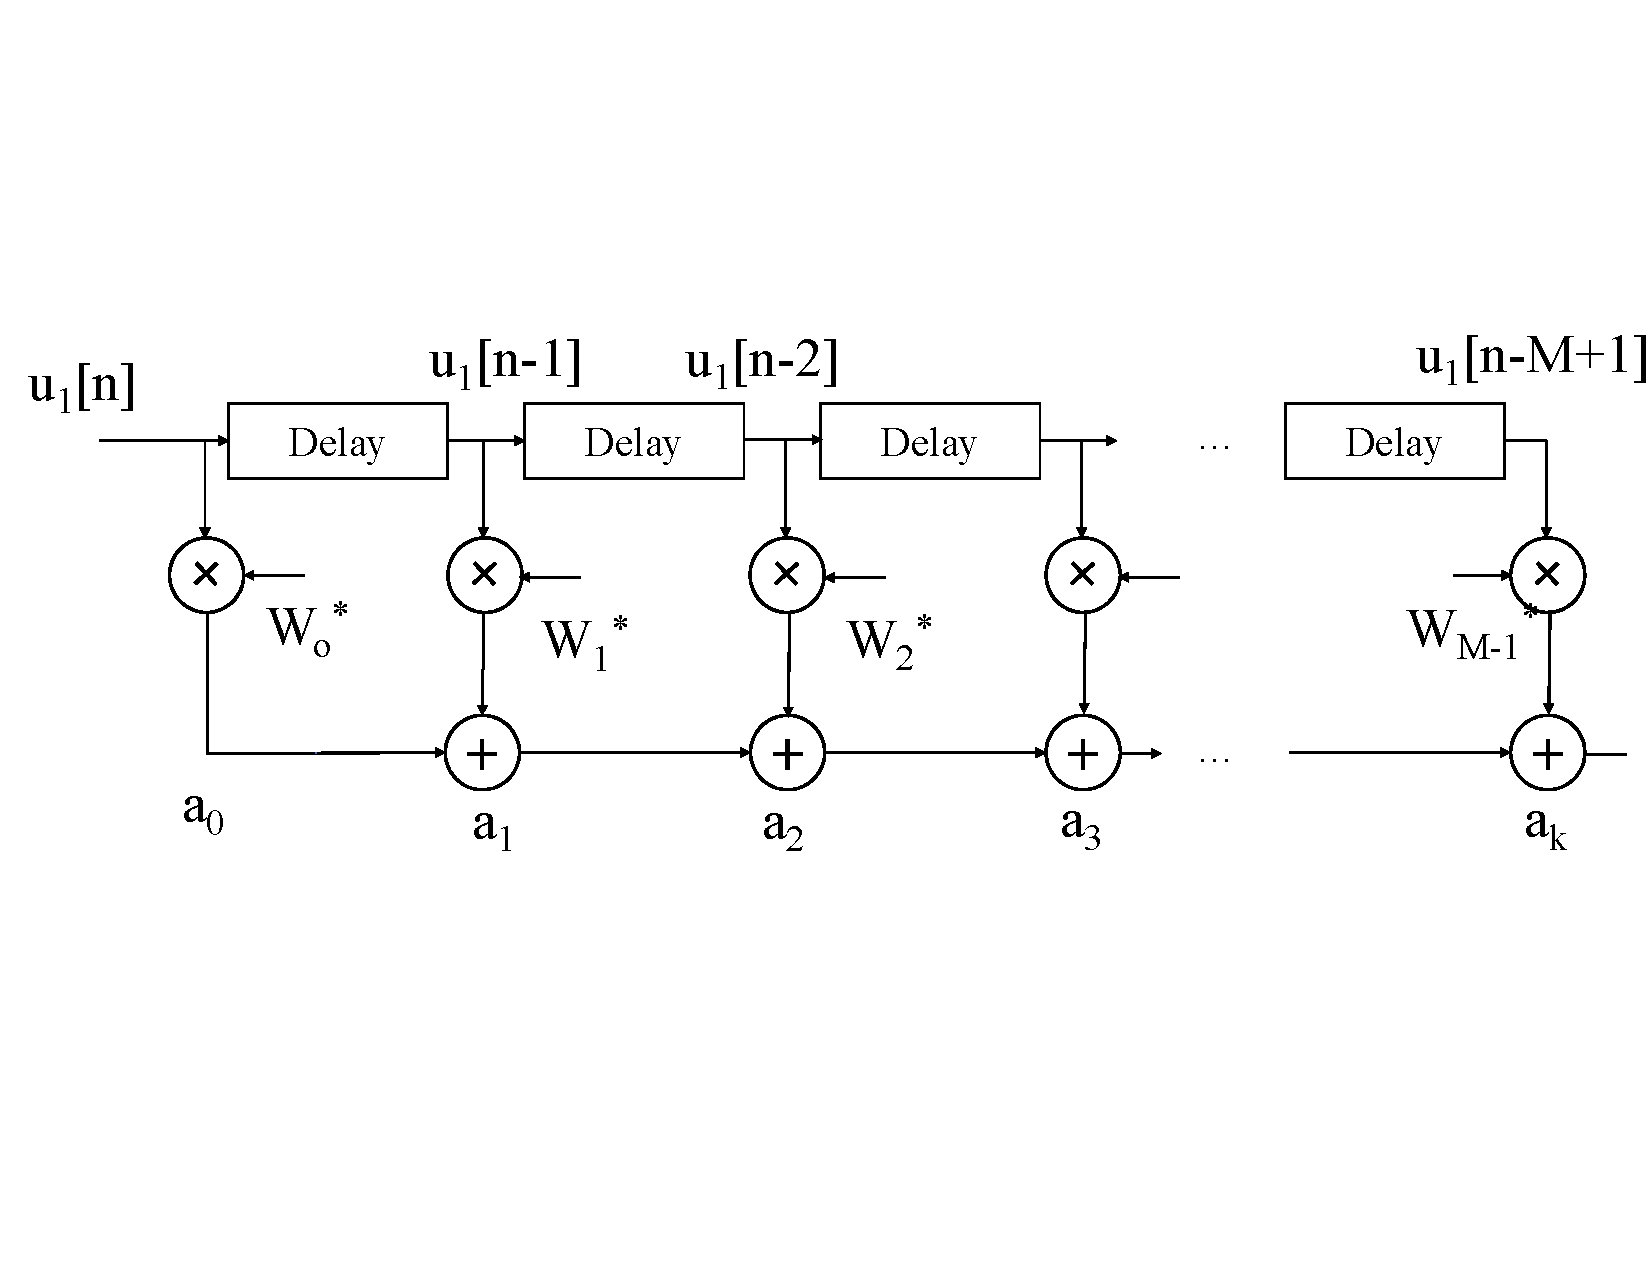
\includegraphics[scale=0.65, trim=0cm 7cm 0cm 3cm, clip]{delay_filter2.pdf}
	\caption{stable, finite response}
	\label{delay2} 
\end{figure}

\begin{doublespace}
$\vec{w}= \left[\begin{array}{c}
w_0\\ w_1\\ .\\.\\. \\ w_{M-1}
\end{array}\right] \in \mathbb{C}^{M\times 1}$; \qquad $\vec{w}^*= \left[\begin{array}{c}
w_0^*\\ w_1^*\\ .\\.\\. \\ w_{M-1}^*
\end{array}\right]$\\ \\
$\vec{w}^T= \left[\begin{array}{c c c c}
w_0& w_1& ...&w_{M-1}
\end{array}\right]$\\
$(\vec{w}^T)^*=(\vec{w}^*)^T= \vec{w}^H$\\

$\vec{u}[n]= \left[\begin{array}{c}
u[n]\\ u[n-1]\\ .\\.\\. \\ u[n-M+1]
\end{array}\right] \in \mathbb{C}^{M\times 1}$\\ \\
$y[n]= \vec{w}^H \cdot \vec{u}[n] = u[n]w_0^*+ u[n-1]w_1^* + ... + u[n-M+1]w_{M-1}^*$\\
$y^*[n]= (\vec{w}^H\vec{u}[n])^*= (( \vec{w}^H \vec{u}[n])^T)^*= (\vec{w}^H \vec{u}[n])^H= \vec{u}^H[n]\vec{w}$\\ \\
$\vec{y}[n]= \left[\begin{array}{c}
	\vec{y}[n]\\ \vec{y}[n+1]\\ .\\.\\. \\ \vec{y}[n+N]
\end{array}\right]\in \mathbb{C}^{(N+1)\times 1}$\\ \\

$\vec{d}[n]= \left[\begin{array}{c}
d[n]\\ d[n+1]\\ .\\.\\. \\ \d[n+N]
\end{array}\right]\in \mathbb{C}^{(N+1)\times 1} \qquad \vec{d} $ is the desired signal\\ \\ \ \\
\textbf{error:} $\vec{e}[n]= \vec{d}[n]-\vec{y}[n]$\\ \ \\
$\vec{w}_{MMSE}= arg \min\limits_{\vec{w}} \underbrace{\sum_{k=0}^{N}|e[n+k]|^2}_{\vec{e}^H[n]\vec{e}[n]= ||\vec{e}[n]||_2^2 \quad \textrm{Squared Euclidean Norm}} $\\ \ \\
Note: MMSE means Minimum Mean Square Error \qquad $\vec{w}$ is the weighting coefficient\\
$\vec{w}_{LS}= arg  \min\limits_{\vec{w}} E[||\vec{e}[n]||_2^2]$ \qquad Note: LS means Least Square Error\\
$\vec{w}_{OPT}= arg  \min\limits_{\vec{w}}  E[||\vec{e}[n]||_2^2]$,\quad  such that \quad $\left\lbrace \begin{array}{l} \vec{w}_1^H\vec{a}_i=b_1\\ i \in \{1,2,...,k\} \end{array} \right.$ Constraints\\ 
OPT means Additional Constraints, Optimization.\\

$\vec{e}^*[n] = \vec{d}^*[n]-\vec{y}^*[n] = \vec{d}^*[n] -\underbrace{\left[\begin{array}{c}
\vec{u}^H[n] \\ \vec{u}^H[n+1] \\ \svdots \\ \vec{u}^H[n+N] \end{array}\right]}_{\text{Signal Matrix }\ma{U}^H[n]} \vec{w} = \vec{d}^*[n]-\ma{U}^H[n]\vec{w}$\\
  
\begin{tabular}{lll}
$||\vec{e}[n]||^2_2=$&$\vec{e}^H[n]\vec{e}[n]$ &$=(\vec{e}^H[n]\vec{e}[n])^*$ (\footnotesize Note: It's a real number, so complex conjungation doesn't hurt!\normalsize) \\
 &&$= (\vec{e}^*[n])^H\vec{e}^*[n]= (\vec{d}^*[n]+\ma{U}^H\vec{w})^H(\vec{d}^*[n]-\ma{U}^H[n]\vec{w})$\\
 &&$= ((\vec{d}^*[n]^H-\vec{w}^H\ma{U}[n])(\vec{d}^*[n]-\ma{U}^H[n]\vec{w}))$\\
 &&$= ||\vec{d}^*[n]||^2_2 -\underbrace{(\vec{d}^*[n])^H\ma{U}^H[n]}_{\vec{\rho^H}}\vec{w}-\vec{w}^H\underbrace{\ma{U}[n]\vec{d}^*[n]}_{\vec{\rho}}+\vec{w}\underbrace{\ma{U}[n]\ma{U}^H[n]}_{\ma{R}=\ma{R}^H}\vec{w}$\\
\end{tabular}
\end{doublespace}
\mybox{Minimization of quadratic forms\\ $||\vec{e}[n]||^2_2=\vec{w}^H\ma{R}\vec{w}- \vec{\rho}^H\vec{w}-\vec{w}^H\vec{\rho}+||\vec{d}[n]||^2_2 \qquad \in \mathbb{R}$ }
\subsubsection{Spatial Filtering}
\paragraph{Planar wave}
\begin{figure}[H]
	\centering
	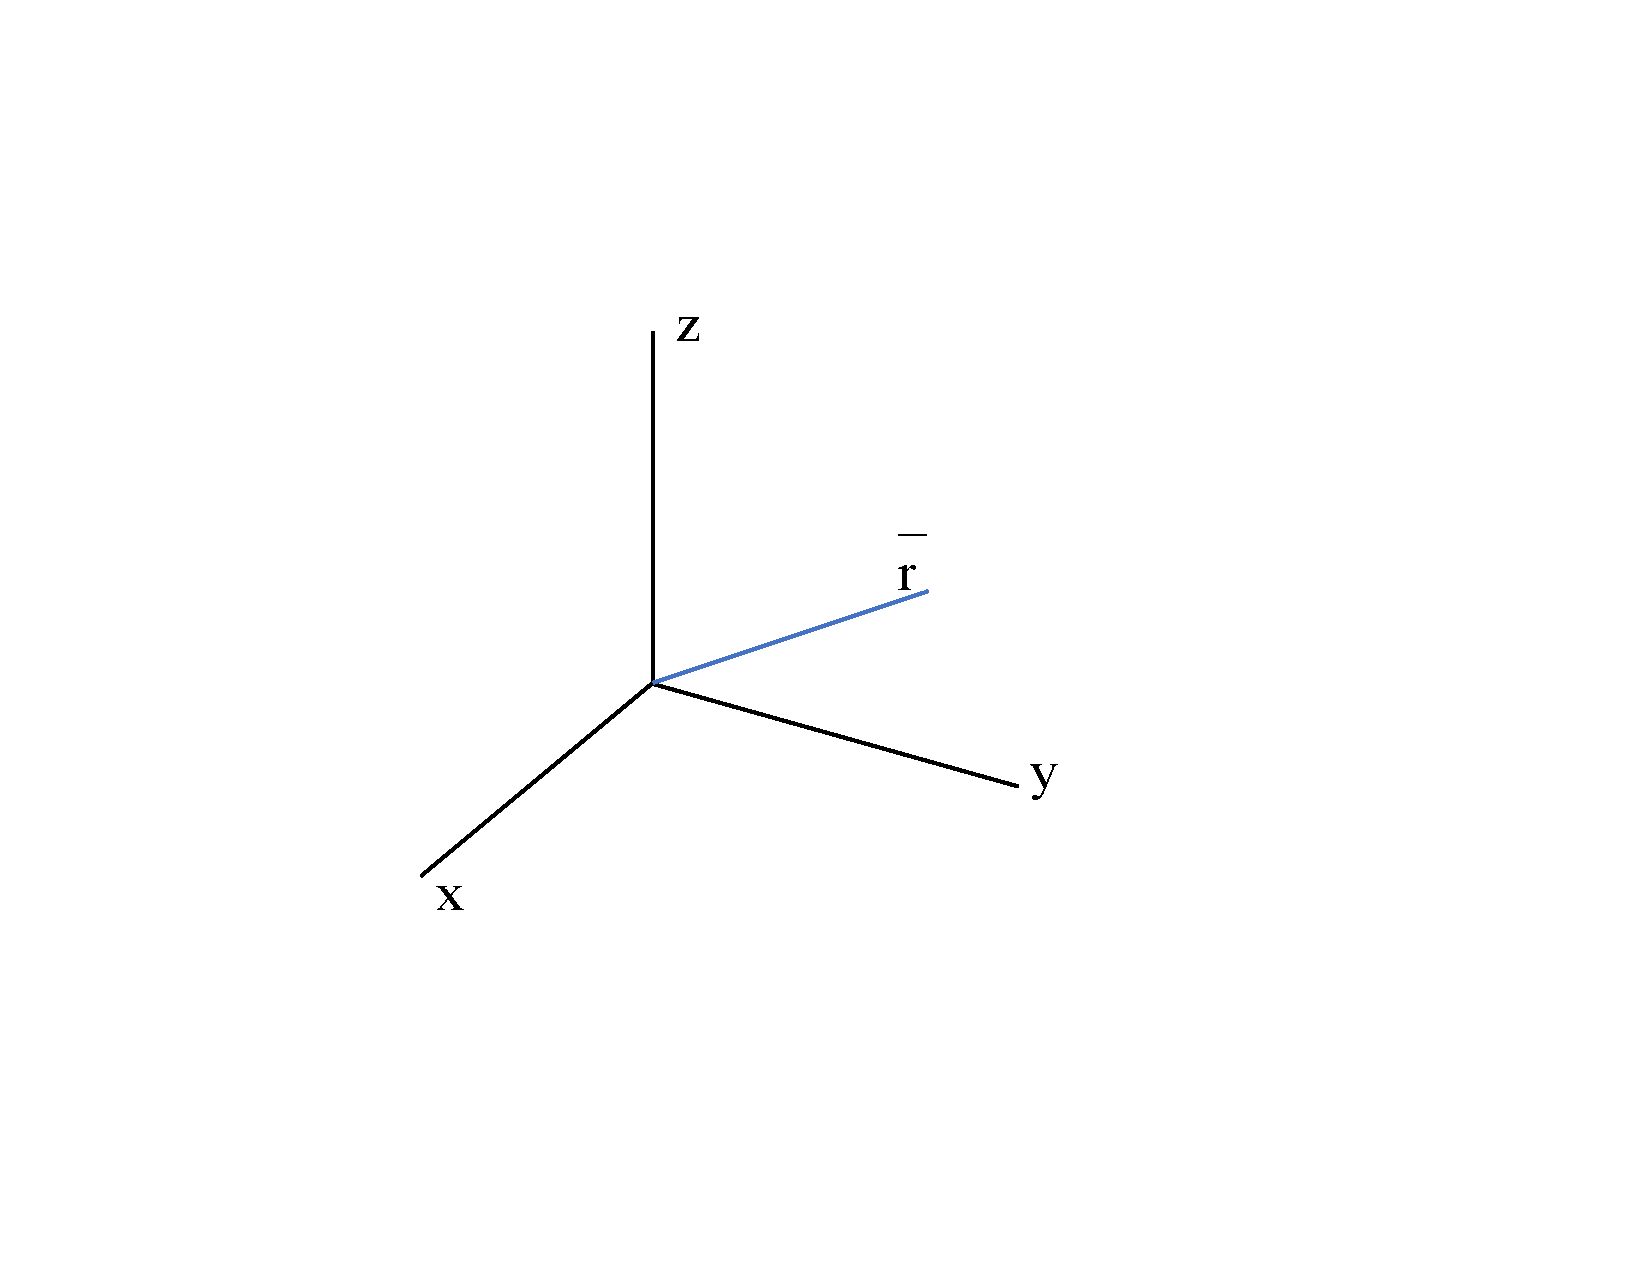
\includegraphics[scale=0.65, trim=0cm 5cm 0cm 4cm, clip]{planarwave.pdf}
	\caption{Direction of planar wave}
	\label{planarwave} 
\end{figure}
$\underbrace{q(t,\vecp{r})}_{field}=F(t-\frac{\vecp{n}\cdot \vecp{r}}{c})$\\
$\vecp{n}\cdot \vecp{n}=1; \quad c=const >0 \qquad$ \vecp{n}= direction of propagation\\ \ \\
\textbf{Property 1}\\
$\forall \Delta \vecp{r}: \Delta \vecp{r} \cdot \vecp{n} = 0 \quad \pfeil q(t,\vecp{r}+\Delta \vecp{r})= q(t,\vecp{r})$\\
"Planar"
\begin{figure}[H]
	\centering
	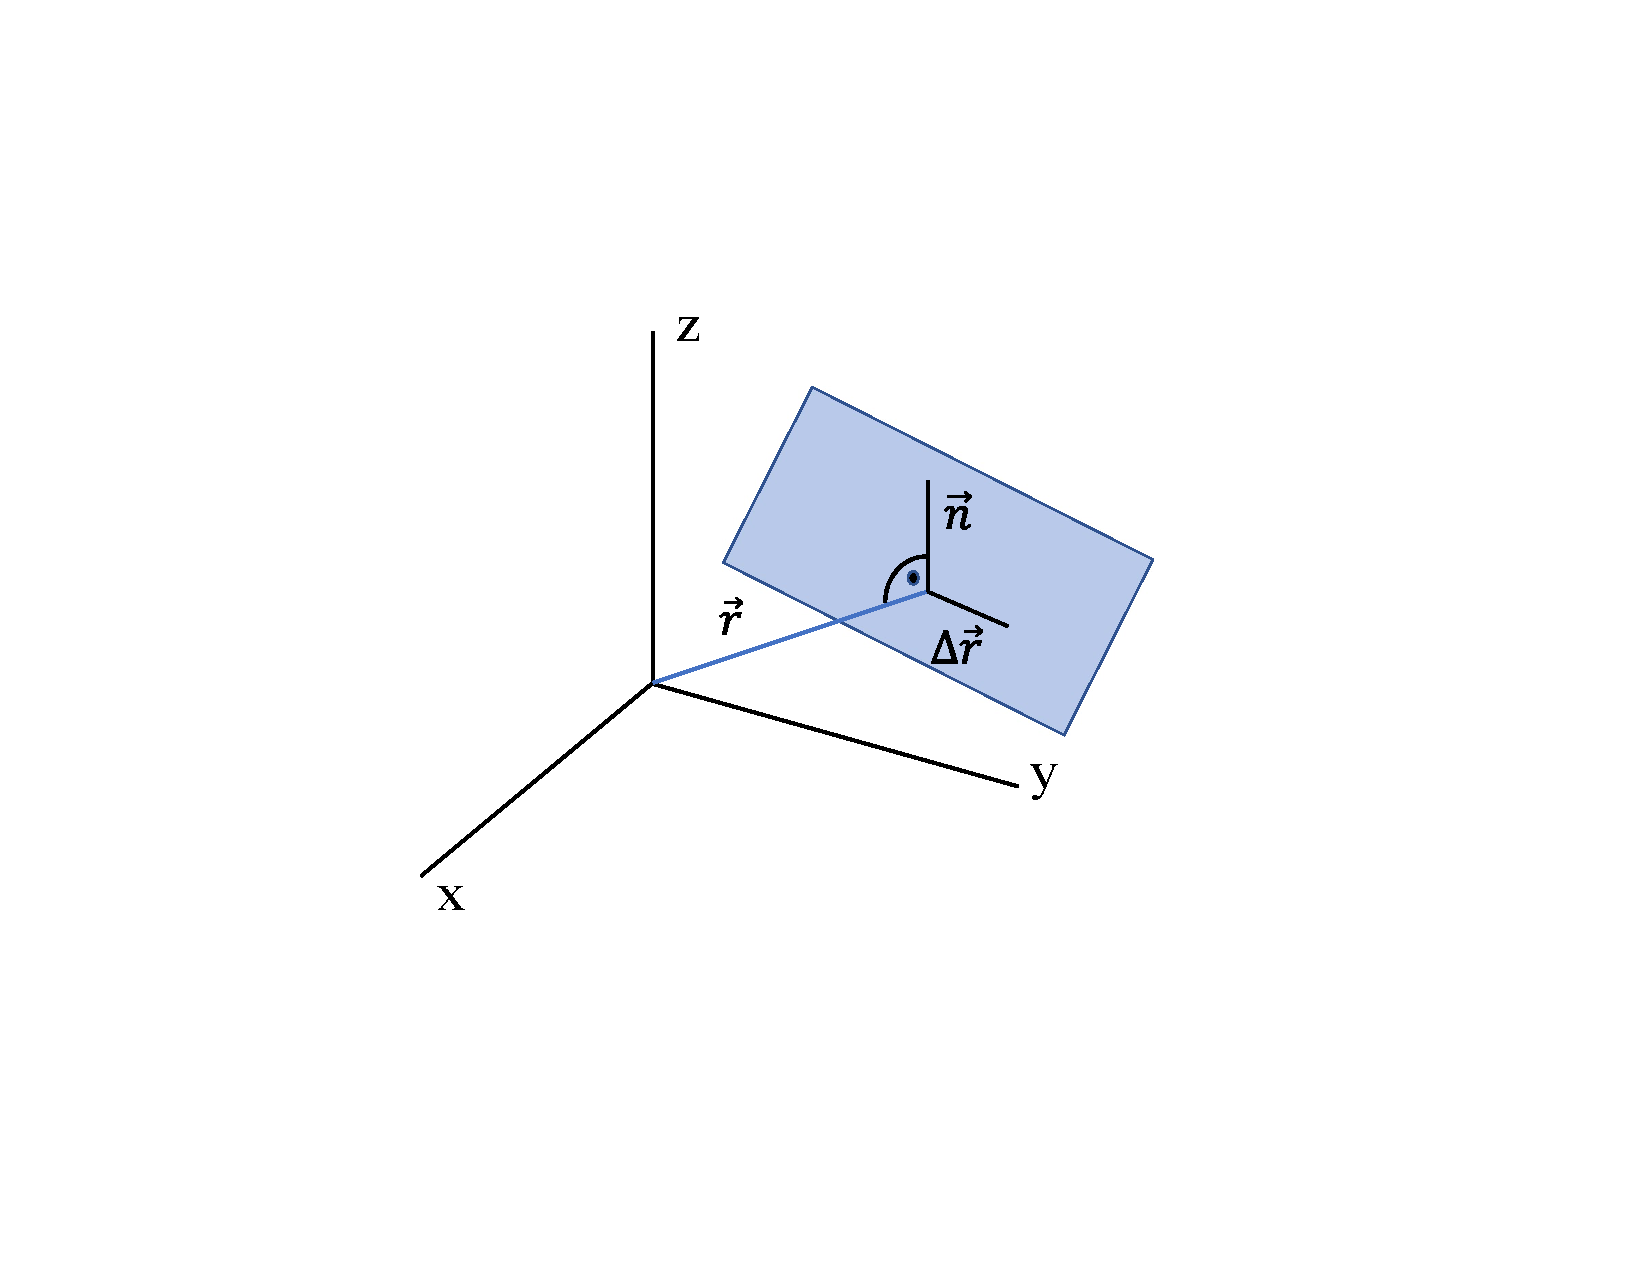
\includegraphics[scale=0.65, trim=0cm 5cm 0cm 4cm, clip]{plane.pdf}
	\caption{plane in space}
	\label{plane} 
\end{figure}

\textbf{Property 2}\\
\begin{doublespace}
$q(t+\Delta t, \vecp{r} + \Delta t\cdot c \vecp{n}) \equiv q(t,\vecp{r})$\\
Moving of $q(t,\vecp{r})$ into direction of $\vecp{n}$ with speed $c$.\\

\texttt{Harmonic planar wave:}\\
$F(\tau)= A \cos(2\pi f_0\tau +\varphi ) \qquad A, f_0, \varphi = const.$\\ 
$q(t,\vecp{r})= A \cos(2\pi f_0(t-\frac{\vecp{n}\cdot\vecp{r}}{c})+\varphi) = \Re{u(\vecp{r})e^{(j2\pi f_0t)}}$\\
$u(\vecp{r})= \underbrace{A e^{(j\varphi)}}_{S \in \mathbb{C}; s = const.} e^{(-j2\pi f_0 \frac{\vecp{n}\cdot\vecp{r}}{c})}$\\ \ \\
\textbf{Property 3}\\
$u(\vecp{r}+ \frac{c}{f_0}\vecp{n})\equiv u(\vecp{r})$ \qquad $\lambda$ wave length; $\lambda =\frac{c}{f_0} $\\ \ \\
$u(\vecp{r}) = s\cdot  e^{-j2\pi \frac{\vecp{n}\cdot\vecp{r}}{\lambda}}$\\ \ \\


$u(\vecp{r}+ l\vec{n})= u(\vecp{r})\cdot e^{-j2\pi \frac{l}{\lambda}}$\\
Phase shift, if you go into direction of wave propagation\\ \ \\ \ \\
\texttt{Modulated harmonic planar wave}\\
s is no longer constant\\
$s= s(t,\vecp{r})= s(t-\frac{\vecp{n}\cdot\vecp{r}}{c})$ \qquad remain wave \\
\end{doublespace}
\mybox{$u(\vecp{r},t)=s(t-\frac{\vecp{n}\cdot\vecp{r}}{c})e^{(-j2\pi \frac{\vecp{n}\cdot \vecp{r}}{\lambda})}$ }\\ \ \\

\subsubsection{Spatial Sampling}
\begin{doublespace}

\begin{figure}[H]
	\centering
	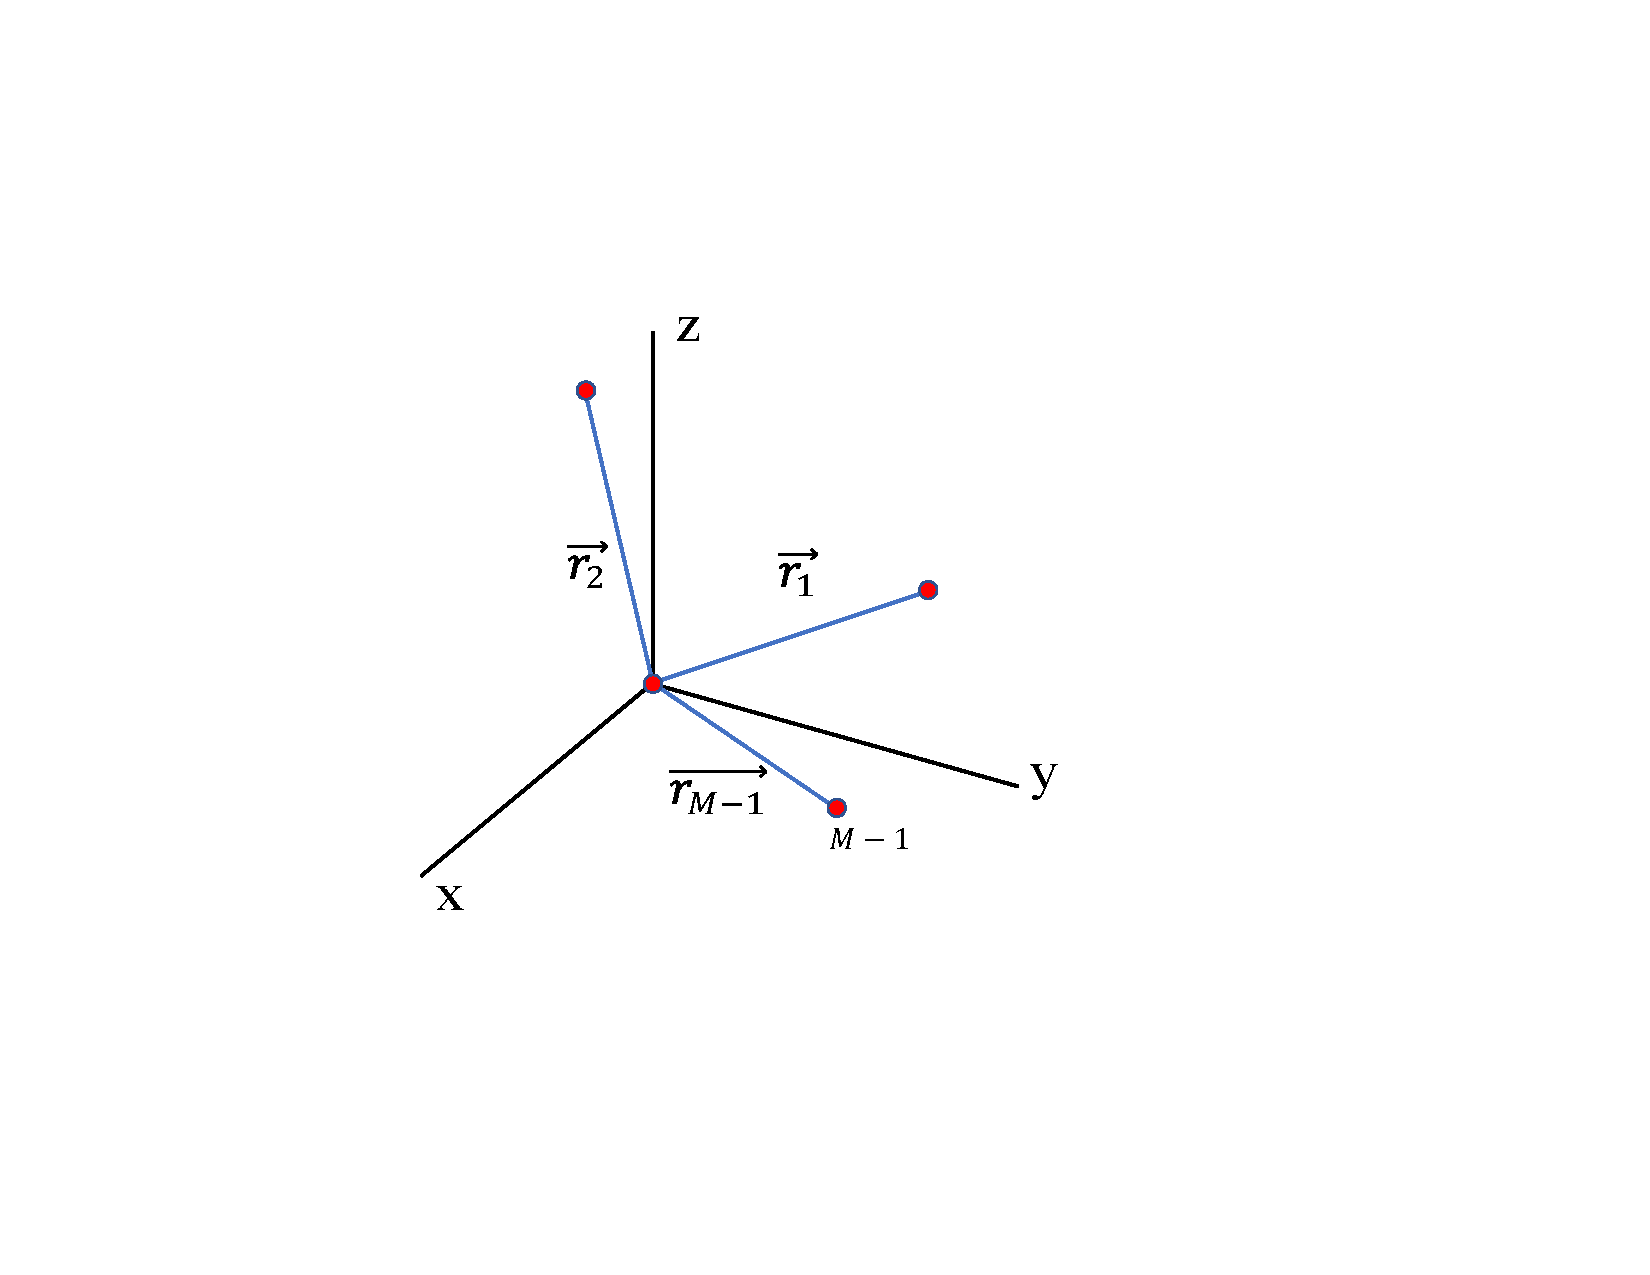
\includegraphics[scale=0.65, trim=0cm 6cm 0cm 5cm, clip]{spatialsampling.pdf}
	\caption{Spatial Sampling with M sensors}
	\label{sampling} 
\end{figure}
$\vec{u}[t]= \left[\begin{array}{c}
s(t)\\ s(t-\frac{\vecp{n}\cdot\vecp{r}_1}{c})e^{-j2\pi \frac{\vecp{n}\cdot \vecp{r}_1}{\lambda}}\\ \svdots \\s(t-\frac{\vecp{n}\cdot \vecp{r}_{M-1}}{c})e^{-j2\pi \frac{\vecp{n}\cdot \vecp{r}_{M-1}}{\lambda}} 
\end{array}\right] $\pfeil Sensor array (receive vector)\\ \ \\
Definition coherence: Coherence (physics), an ideal property of waves that enables stationary (i.e. temporally and spatially constant) interference.
\begin{itemize}
	\item coherence distance, length $l_{coh}$\\
				if $|l|\leq l_{coh} \iff s(t) \approx s(t-\frac{l}{c})$ \\
	\item assume all sensors within coherence distance. \\
$\vec{u}(t)\approx s(t) \underbrace{\left[\begin{array}{c}
	1\\ e^{-j2\pi \frac{\vecp{n}\cdot \vecp{r}_1}{\lambda}}\\ \svdots \\ e^{-j2\pi \frac{\vecp{n}\cdot \vecp{r}_{M-1}}{\lambda}}
	\end{array}\right] }_{\vec{a}(\vecp{n})  \text{ Array steering Vector}} $ \pfeil no time delay, only phase shifts
\end{itemize}
$\vec{u}(nT)=s[n]\cdot \vec{a}(\vecp{n})$\with T$=$ Sampling Time, n $=$ Sampling Index $\neq \vecp{n}$ \\
\texttt{Example:}\\
$f_0 = 2.6 GHz\qquad B=20MHz$\\
$\frac{l_{coh}}{c}<< \frac{1}{B}, \quad \frac{l_{coh}}{c}\approx\frac{1}{30B}, \quad \lambda = \frac{c}{f_0}$  \\ $l_{coh}\approx 0.5m \approx 4\lambda$\\ $u[n]$ 
\end{doublespace}

\subsubsection{Large Array}
\begin{doublespace}
$s[n-\underbrace{\frac{\tau_i}{T}}_{\text{fractioned Delay}}]= s(nT-\tau_i)\qquad \tau_i=\frac{\vecp{n}\cdot\vecp{r_i}}{c}$\\ \\
\[ s[n-\frac{\tau_i}{T}]\approx  \sum_{K=-L_1}^{L_2} a_{i,k}  \quad s[n-k]\]\\ \\
$\vec{u}[n]= \underbrace{ \begin{bmatrix}1&0&\shdots&0\\0&e^{-j2\pi \frac{\vecp{n}\cdot\vecp{r}_1}{\lambda}} \\\svdots& &\ddots&\\ 0 & \shdots &e^{-j2\pi \frac{\vecp{n}\cdot\vecp{r}_{M-1}}{c}} \end{bmatrix} 
\begin{bmatrix}\overbrace{0,...,0,}^{L_1} & 1 & \overbrace{0,...,0,}^{L_2} \\ a_{1,-L_1} & ... & a_{1,-L_2}\\ \svdots & ... & \svdots \\ a_{M-1,-L_1}& ... &a_{M-1,-L_2}\end{bmatrix}}_{\ma{A}\vecp{n}} \underbrace{\begin{bmatrix}s[n+L_1]\\ s[n+L_1-1] \\\svdots \\ s[n-L_2] \end{bmatrix}}_{\vec{s}[n]}$ \\ \ \\
$\vec{u}[n]= \ma{A}(\vec{n}) \cdot\vec{s}[n]$ \pfeil long array\\
$u[n] = \vec{a}(\vecp{n})\cdot s[n]$ \pfeil small array\\
\end{doublespace}

\subsubsection{Uniform Linear Array, ULA}
same distance in between sensors, all in one line\\

\begin{figure}[H]
	\centering
	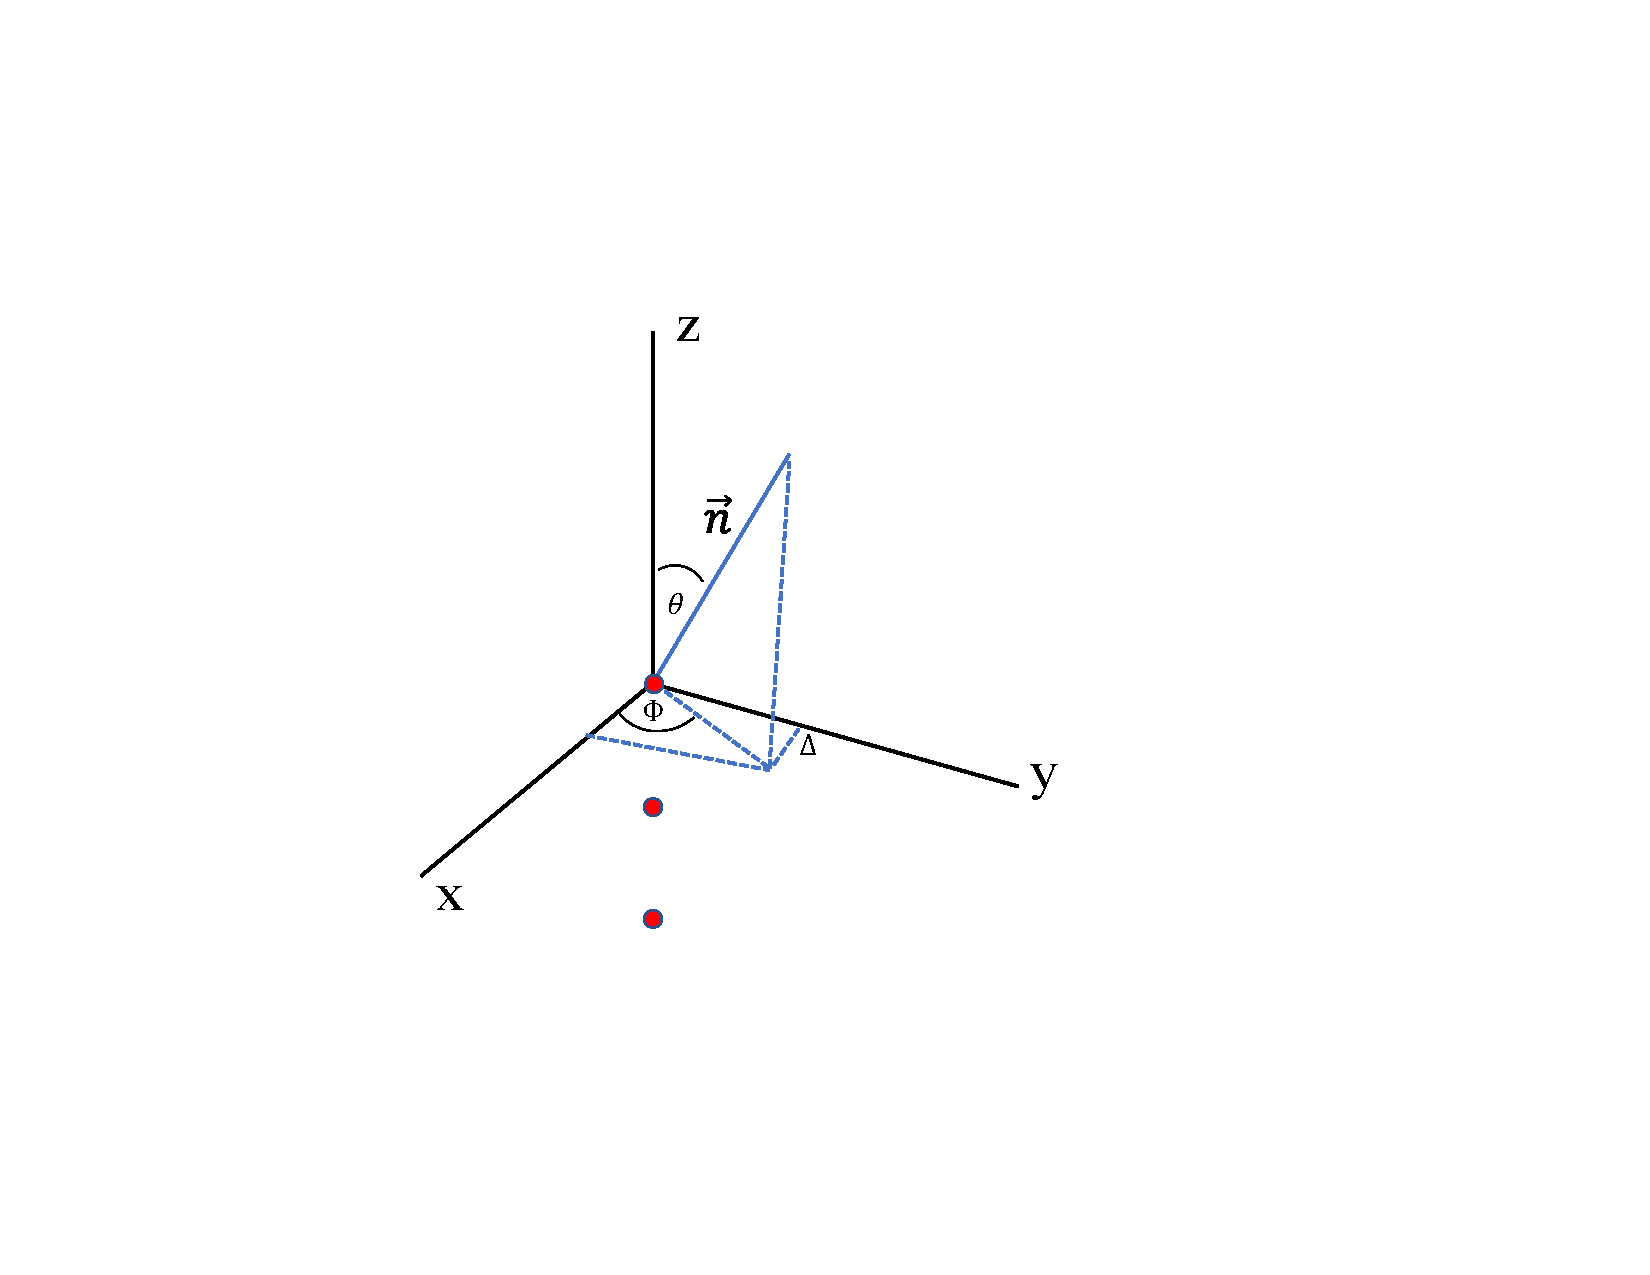
\includegraphics[scale=0.65, trim=0cm 5cm 0cm 4cm, clip]{ULA.pdf}
	\caption{Uniform Linear Array}
	\label{ula} 
\end{figure}
\begin{doublespace}
$\vecp{r}_i = -\vecp{e}_z \Delta i$ \qquad $i \in \{0,1,...,M-1\}$\\ \\
$\vecp{r}= r \begin{bmatrix}
cos \varphi sin \theta\\ sin \varphi sin \theta \\ cos \theta
\end{bmatrix}$ \qquad spherical coordinates in cartesian vector  \\ \\
$\vecp{n}=-\frac{\vecp{r}}{r}, \qquad \vecp{n}\cdot \vecp{n}=1$\\
$\vecp{r}_i\cdot\vecp{n}= - \Delta i (-\cos \Theta)= cos\Theta \cdot\Delta\cdot i$\\ \\ 
$\vec{a}(\vecp{n})= \vec{a}(\Theta)= \begin{bmatrix}1 \\ e^{-j2\pi \frac{\Delta}{\lambda}cos \Theta}\\e^{-j2\pi \frac{2\Delta}{\lambda}cos \Theta}\\ \svdots \\ e^{-j2\pi \frac{(M-1)\Delta}{\lambda}cos \Theta} \end{bmatrix}$ \qquad \pfeil Van Der Monde-Vector\\ (ULA Steering Vector)\\ \\
\end{doublespace}

\begin{figure}[H]
	\centering
	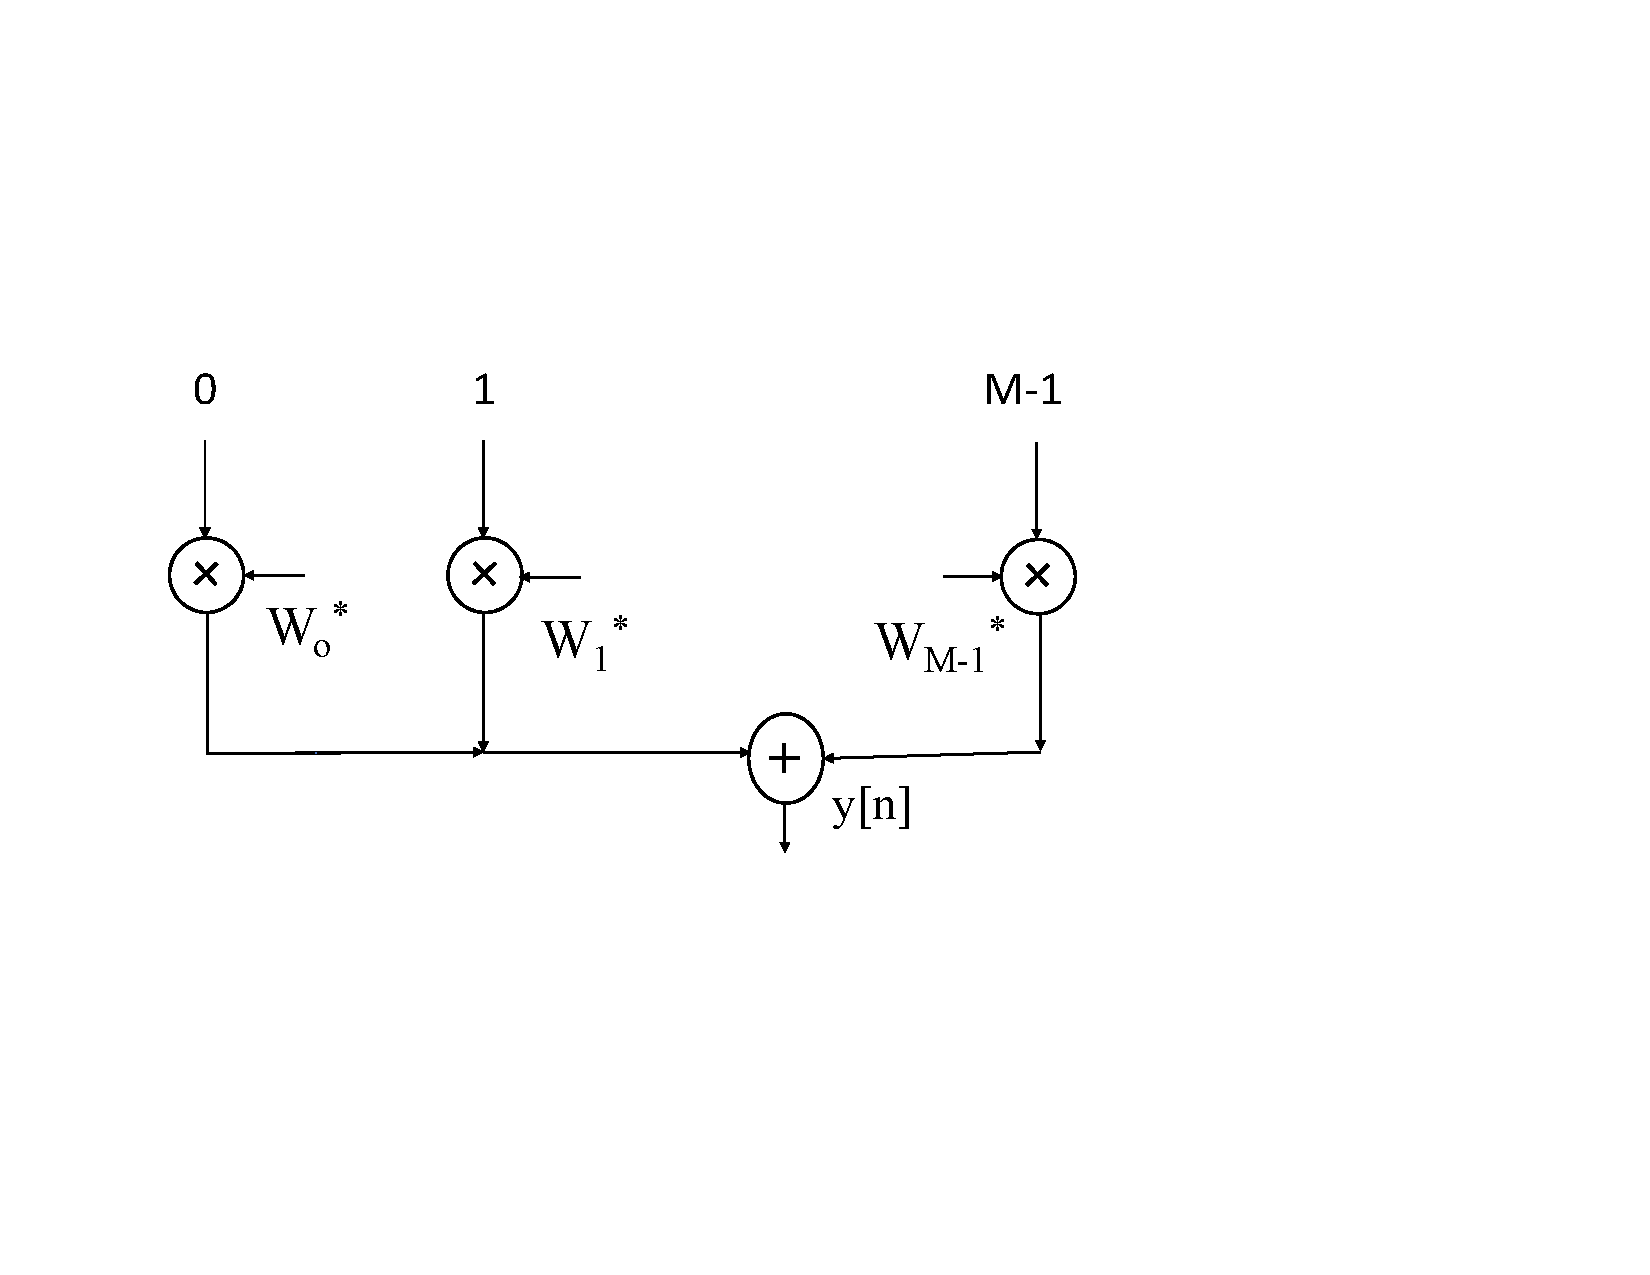
\includegraphics[scale=0.55, trim=0cm 7cm 5cm 4cm, clip]{summe.pdf}
	\caption{Sensors, figure \ref{ula}}
	\label{summe} 
\end{figure}
\begin{doublespace}
$y[n]= \vec{w}^H \vec{u}[n]$\\
$y[n]^*= \vec{u}^H[n] \vec{w}$\\ \ \\
$y^*[n] = \begin{bmatrix}y^*[n]\\ y^*[n-1]\\ \svdots \\ y^*[n+N]\end{bmatrix} = \underbrace{\begin{bmatrix}\vec{u}^H[n]\\ \vec{u}^H[n+1]\\ \svdots\\ \vec{u}^H[n+N]\end{bmatrix}}_{\ma{U}^H[n]}\vec{w}= \ma{U}^H[n]\vec{w}$\\ \\
$\vec{u}[n]= \underbrace{\vec{a}(\Theta) s[n]}_{desired signal}+ \underbrace{\vec{\eta}[n]}_{\text{interference + noise}}$\\ \\
Constraint: $\vec{w}^H \vec{a}(\Theta)=1$\\
$y[n]=\vec{w}^H \vec{u}[n] = \vec{w}^H(\vec{a}(\Theta) s[n]+ \vec{\eta}[n])= \underbrace{\vec{w}^H\vec{a}(\Theta)}_1s[n]+ \vec{w}^H\vec{\eta}[n]= s[n] + \vec{w}^H\vec{\eta}[n]$\\\\
$\underset{\vec{w}}{min} \quad ||y[n]||_F^2$ \quad such that $\vec{w}^H \vec{a}(\Theta)=1$\\
\begin{tabular}{ll}
$||y[n]||_2^2$ &$= \vec{y}^H[n]\vec{y}[n]$\\
 &$=(\vec{y}^*[n])^H(\vec{y}[n]) \in \mathbb{R}$\\
 &$= (\ma{U}^H[n]\vec{w})^H(\ma{U}^H[n]\vec{w})$\\
 &$= \vec{w} \underbrace{\ma{U}[n]\ma{U}^H[n]}_{\ma{R}}{\vec{w}}= \vec{w}^H\ma{R}\vec{w}$\\
\end{tabular}
\end{doublespace}
\mybox{$\vec{w}_{OPT}= arg \min\limits_{\vec{w}} \vec{w}^H\ma{R}\vec{w}$, \qquad s.t. \quad $\vec{w}^H\vec{a}(\Theta)=1$}


\newpage